\chapter{Quantum computing}\label{quantumchap}

\begin{objectives} \label[objectives]{See-main-aspects-in-which}

\begin{itemize}
\tightlist
\item
  See main aspects in which quantum mechanics differs from local
  deterministic theories.\\
\item
  Model of quantum circuits, or equivalently QNAND-CIRC programs\\
\item
  The complexity class \(\mathbf{BQP}\) and what we know about its
  relation to other classes\\
\item
  Ideas behind Shor's Algorithm and the Quantum Fourier Transform
\end{itemize}

\end{objectives}

\begin{quote}
\emph{``We always have had (secret, secret, close the doors!) \ldots{} a
great deal of difficulty in understanding the world view that quantum
mechanics represents \ldots{} It has not yet become obvious to me that
there's no real problem. \ldots{} Can I learn anything from asking this
question about computers--about this may or may not be mystery as to
what the world view of quantum mechanics is?''} , Richard Feynman, 1981
\end{quote}

\begin{quote}
\emph{``The only difference between a probabilistic classical world and
the equations of the quantum world is that somehow or other it appears
as if the probabilities would have to go negative''}, Richard Feynman,
1981
\end{quote}

There were two schools of natural philosophy in ancient Greece.
\emph{Aristotle} believed that objects have an \emph{essence} that
explains their behavior, and a theory of the natural world has to refer
to the \emph{reasons} (or ``final cause'' to use Aristotle's language)
as to why they exhibit certain phenomena. \emph{Democritus} believed in
a purely mechanistic explanation of the world. In his view, the universe
was ultimately composed of elementary particles (or \emph{Atoms}) and
our observed phenomena arise from the interactions between these
particles according to some local rules. Modern science (arguably
starting with Newton) has embraced Democritus' point of view, of a
mechanistic or ``clockwork'' universe of particles and forces acting
upon them.

While the classification of particles and forces evolved with time, to a
large extent the ``big picture'' has not changed from Newton till
Einstein. In particular it was held as an axiom that if we knew fully
the current \emph{state} of the universe (i.e., the particles and their
properties such as location and velocity) then we could predict its
future state at any point in time. In computational language, in all
these theories the state of a system with \(n\) particles could be
stored in an array of \(O(n)\) numbers, and predicting the evolution of
the system can be done by running some efficient (e.g., \(poly(n)\)
time) deterministic computation on this array.

\section{The double slit experiment}\label{The-double-slit-experimen}

Alas, in the beginning of the 20th century, several experimental results
were calling into question this ``clockwork'' or ``billiard ball''
theory of the world. One such experiment is the famous
\href{https://en.wikipedia.org/wiki/Double-slit_experiment}{double slit
experiment}. Here is one way to describe it. Suppose that we buy one of
those baseball pitching machines, and aim it at a soft plastic wall, but
put a \emph{metal barrier with a single slit} between the machine and
the plastic wall (see \cref{doublebaseballfig}). If we shoot baseballs
at the plastic wall, then some of the baseballs would bounce off the
metal barrier, while some would make it through the slit and dent the
wall. If we now carve out an additional slit in the metal barrier then
more balls would get through, and so the plastic wall would be
\emph{even more dented}.


\begin{marginfigure}
\centering
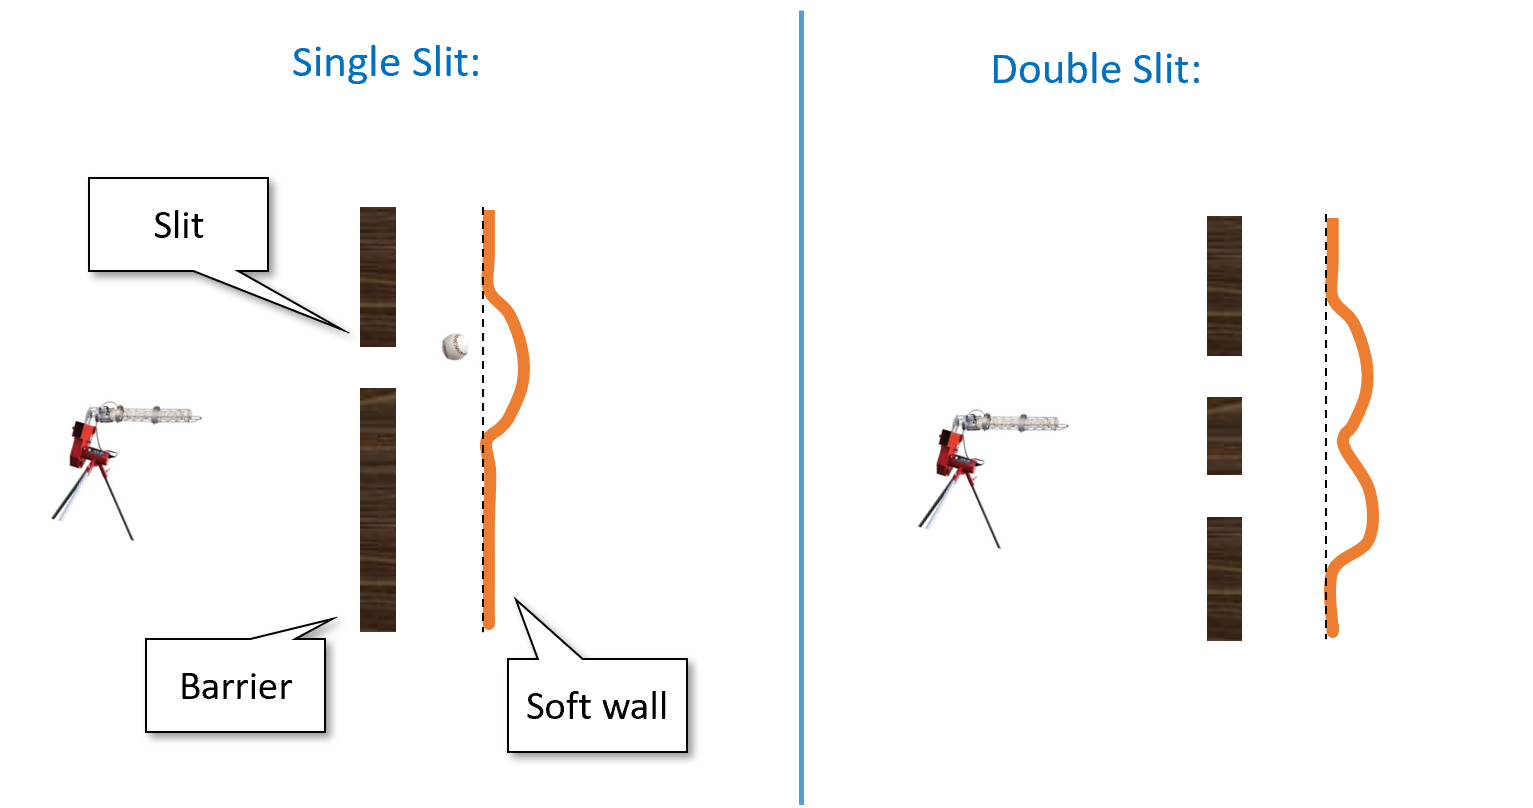
\includegraphics[width=\linewidth, height=1.5in, keepaspectratio]{../figure/double_baseball2.png}
\caption{In the ``double baseball experiment'' we shoot baseballs from a
gun at a soft wall through a hard barrier that has one or two slits open
in it. There is only ``constructive interference'' in the sense that the
dent in each position in the wall when both slits are open is the sum of
the dents when each slit is open on its own.}
\label{doublebaseballfig}
\end{marginfigure}

So far this is pure common sense, and it is indeed (to my knowledge) an
accurate description of what happens when we shoot baseballs at a
plastic wall. However, this is not the same when we shoot
\emph{photons}. Amazingly, if we shoot with a ``photon gun'' (i.e., a
laser) at a wall equipped with photon detectors through some barrier,
then (as shown in \cref{doubleslitfig}) in some positions of the wall we
will see \emph{fewer} hits when the two slits are open than when only
one of them is!. In particular there are positions in the wall that are
hit when the first slit is open, hit when the second gun is open, but
are \emph{not hit at all when both slits are open!}.


\begin{marginfigure}
\centering
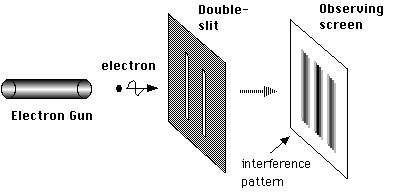
\includegraphics[width=\linewidth, height=1.5in, keepaspectratio]{../figure/double-slit-setup.PNG}
\caption{The setup of the double slit experiment in the case of photon
or electron guns. We see also \emph{destructive} interference in the
sense that there are some positions on the wall that get \emph{fewer}
hits when both slits are open than they get when only one of the slits
is open. See also
\href{https://www.youtube.com/watch?v=DfPeprQ7oGc}{this video}.}
\label{doubleslitfig}
\end{marginfigure}

It seems as if each photon coming out of the gun is aware of the global
setup of the experiment, and behaves differently if two slits are open
than if only one is. If we try to ``catch the photon in the act'' and
place a detector right next to each slit so we can see exactly the path
each photon takes then something even more bizarre happens. The mere
fact that we \emph{measure} the path changes the photon's behavior, and
now this ``destructive interference'' pattern is gone and the number of
times a position is hit when two slits are open is the sum of the number
of times it is hit when each slit is open.

\begin{pause} \label[pause]{You-should-read-the-parag}

You should read the paragraphs above more than once and make sure you
appreciate how truly mind boggling these results are.

\end{pause}

\section{Quantum amplitudes}\label{Quantum-amplitudes}

The double slit and other experiments ultimately forced scientists to
accept a very counterintuitive picture of the world. It is not merely
about nature being randomized, but rather it is about the probabilities
in some sense ``going negative'' and cancelling each other!

To see what we mean by this, let us go back to the baseball experiment.
Suppose that the probability a ball passes through the left slit is
\(p_L\) and the probability that it passes through the right slit is
\(p_R\). Then, if we shoot \(N\) balls out of each gun, we expect the
wall will be hit \((p_L+p_R)N\) times. In contrast, in the quantum world
of photons instead of baseballs, it can sometimes be the case that in
both the first and second case the wall is hit with positive
probabilities \(p_L\) and \(p_R\) respectively but somehow when both
slits are open the wall (or a particular position in it) is not hit at
all. It's almost as if the probabilities can ``cancel each other out''.

To understand the way we model this in quantum mechanics, it is helpful
to think of a ``lazy evaluation'' approach to probability. We can think
of a probabilistic experiment such as shooting a baseball through two
slits in two different ways:

\begin{itemize}
\item
  When a ball is shot, ``nature'' tosses a coin and decides if it will
  go through the left slit (which happens with probability \(p_L\)),
  right slit (which happens with probability \(p_R\)), or bounce back.
  If it passes through one of the slits then it will hit the wall. Later
  we can look at the wall and find out whether or not this event
  happened, but the fact that the event happened or not is determined
  independently of whether or not we look at the wall.
\item
  The other viewpoint is that when a ball is shot, ``nature'' computes
  the probabilities \(p_L\) and \(p_R\) as before, but does \emph{not}
  yet ``toss the coin'' and determines what happened. Only when we
  actually look at the wall, nature tosses a coin and with probability
  \(p_L+p_R\) ensures we see a dent. That is, nature uses ``lazy
  evaluation'', and only determines the result of a probabilistic
  experiment when we decide to \emph{measure} it.
\end{itemize}

While the first scenario seems much more natural, the end result in both
is the same (the wall is hit with probability \(p_L+p_R\)) and so the
question of whether we should model nature as following the first
scenario or second one seems like asking about the proverbial tree that
falls in the forest with no one hearing about it.

However, when we want to describe the double slit experiment with
photons rather than baseballs, it is the second scenario that lends
itself better to a quantum generalization. Quantum mechanics associates
a number \(\alpha\) known as an \emph{amplitude} with each probabilistic
experiment. This number \(\alpha\) can be \emph{negative}, and in fact
even \emph{complex}. We never observe the amplitudes directly, since
whenever we \emph{measure} an event with amplitude \(\alpha\), nature
tosses a coin and determines that the event happens with probability
\(|\alpha|^2\). However, the sign (or in the complex case, phase) of the
amplitudes can affect whether two different events have
\emph{constructive} or \emph{destructive} interference.

Specifically, consider an event that can either occur or not
(e.g.~``detector number 17 was hit by a photon''). In classical
probability, we model this by a probability distribution over the two
outcomes: a pair of non-negative numbers \(p\) and \(q\) such that
\(p+q=1\), where \(p\) corresponds to the probability that the event
occurs and \(q\) corresponds to the probability that the event does not
occur. In quantum mechanics, we model this also by pair of numbers,
which we call \emph{amplitudes}. This is a pair of (potentially negative
or even complex) numbers \(\alpha\) and \(\beta\) such that
\(|\alpha|^2 + |\beta|^2 =1\). The probability that the event occurs is
\(|\alpha|^2\) and the probability that it does not occur is
\(|\beta|^2\). In isolation, these negative or complex numbers don't
matter much, since we anyway square them to obtain probabilities. But
the interaction of positive and negative amplitudes can result in
surprising \emph{cancellations} where somehow combining two scenarios
where an event happens with positive probability results in a scenario
where it never does.

\begin{pause} \label[pause]{If-you-dont-find-the-abov}

If you don't find the above description confusing and unintuitive, you
probably didn't get it. Please make sure to re-read the above paragraphs
until you are thoroughly confused.

\end{pause}

Quantum mechanics is a mathematical theory that allows us to calculate
and predict the results of the double-slit and many other experiments.
If you think of quantum mechanics as an explanation as to what
``really'' goes on in the world, it can be rather confusing. However, if
you simply ``shut up and calculate'' then it works amazingly well at
predicting experimental results. In particular, in the double slit
experiment, for any position in the wall, we can compute numbers
\(\alpha\) and \(\beta\) such that photons from the first and second
slit hit that position with probabilities \(|\alpha|^2\) and
\(|\beta|^2\) respectively. When we open both slits, the probability
that the position will be hit is proportional to \(|\alpha+\beta|^2\),
and so in particular, if \(\alpha=-\beta\) then it will be the case
that, despite being hit when \emph{either} slit one or slit two are
open, the position is \emph{not hit at all} when they both are. If you
are confused by quantum mechanics, you are not alone: for decades people
have been trying to come up with
\href{https://en.wikipedia.org/wiki/Interpretations_of_quantum_mechanics}{explanations}
for ``the underlying reality'' behind quantum mechanics, including
\href{https://en.wikipedia.org/wiki/De_Broglie\%E2\%80\%93Bohm_theory}{Bohmian
Mechanics},
\href{https://en.wikipedia.org/wiki/Many-worlds_interpretation}{Many
Worlds} and others. However, none of these interpretations have gained
universal acceptance and all of those (by design) yield the same
experimental predictions. Thus at this point many scientists prefer to
just ignore the question of what is the ``true reality'' and go back to
simply ``shutting up and calculating''.

\hypertarget{complexrem}{}
\begin{remark}[Complex vs real, other simplifications] \label[remark]{complexrem}

If (like the author) you are a bit intimidated by complex numbers, don't
worry: you can think of all amplitudes as \emph{real} (though
potentially \emph{negative}) numbers without loss of understanding. All
the ``magic'' of quantum computing already arises in this case, and so
we will often restrict attention to real amplitudes in this chapter.

We will also only discuss so-called \emph{pure} quantum states, and not
the more general notion of \emph{mixed} states. Pure states turn out to
be sufficient for understanding the algorithmic aspects of quantum
computing.

More generally, this chapter is not meant to be a complete description
of quantum mechanics, quantum information theory, or quantum computing,
but rather illustrate the main points where these differ from classical
computing.

\end{remark}

\subsection{Linear algebra quick
review}\label{Linear-algebra-quick-revi}

\emph{Linear algebra} underlies much of quantum mechanics, and so you
would do well to review some of the basic notions such as vectors,
matrices, and linear subspaces. The operations in quantum mechanics can
be represented as linear functions over the \emph{complex} numbers, but
we stick to the real numbers in this chapter. This does not cause much
loss in understanding but does allow us to simplify our notation and
eliminate the use of the complex conjugate.

The main notions we use are:

\begin{itemize}
\item
  A function \(F:\R^N \rightarrow \R^N\) is \emph{linear} if
  \(F(\alpha u + \beta v) = \alpha F(u) + \beta F(v)\) for every
  \(\alpha,\beta \in \R\) and \(u,v \in \R^N\).
\item
  The \emph{inner product} of two vectors \(u,v \in \R^N\) can be
  defined as \(\langle u,v \rangle = \sum_{i\in [N]} u_iv_i\). (There
  can be different inner products but we stick to this one.) The
  \emph{norm} of a vector \(u \in \R^N\) is defined as
  \(\|u\| = \sqrt{\langle u,u \rangle} = \sqrt{\sum_{i\in [N]}u_i^2}\).
  We say that \(u\) is a \emph{unit vector} if \(\|u\|=1\).
\item
  Two vectors \(u,v \in \R^N\) are \emph{orthogonal} if
  \(\langle u,v\rangle = 0\). An \emph{orthonormal basis} for \(\R^N\)
  is a set of \(N\) vectors \(v_0,v_1,\ldots, v_{N-1}\) such that
  \(\| v_i \|=1\) for every \(i\in [N]\) and
  \(\langle v_i,v_j \rangle=0\) for every \(i\neq j\). A canoncial
  example is the \emph{standard basis} \(e_0,\ldots,e_{N-1}\), where
  \(e_i\) is the vector that has zeroes in all cooordinates except the
  \(i\)-th coordinate in which its value is \(1\). A quirk of the
  quantum mechanics literature is that \(e_i\) is often denoted by
  \(|i \rangle\). We often consider the case \(N=2^n\), in which case we
  identify \([N]\) with \(\{0,1\}^n\) and for every \(x\in \{0,1\}^n\),
  we denote the standard basis element corresponding to the \(x\)-th
  coordinate by \(|x \rangle\).
\item
  If \(u\) is a vector in \(\R^n\) and \(v_0,\ldots,v_{N-1}\) is an
  orthonormal basis for \(\R^N\), then there are coefficients
  \(\alpha_0,\ldots,\alpha_{N-1}\) such that
  \(u = \alpha_0v_0 + \cdots + \alpha_{N-1}v_{N-1}\). Consequently, the
  value \(F(u)\) is determined by the values \(F(v_0)\), \(\ldots\),
  \(F(v_{N-1})\). Moreover,
  \(\|u\| = \sqrt{\sum_{i\in [N]} \alpha_i^2}\).
\item
  We can represent a linear function \(F:\R^N \rightarrow \R^N\) as an
  \(N\times N\) \emph{matrix} \(M(F)\) where the coordinate in the
  \(i\)-th row and \(j\)-th column of \(M(F)\) (that is \(M(F)_{i,j}\))
  is equal to \(\langle e_i , F(e_j) \rangle\) or equivalently the
  \(i\)-th coordinate of \(F(e_j)\).
\item
  A linear function \(F:\R^N \rightarrow \R^N\) such that
  \(\| F(u) \| = \|u \|\) for every \(u\) is called \emph{unitary}. It
  can be shown that a function \(F\) is unitary if and only if
  \(M(F) M(F)^\top = I\) where \(\top\) is the \emph{transpose} operator
  (in the complex case the conjugate transpose) and \(I\) is the
  \(N\times N\) identity matrix that has \(1\)'s on the diagonal and
  zeroes everywhere else. (For every two matrices \(A,B\), we use
  \(A B\) to denote the \emph{matrix product} of \(A\) and \(B\).)
  Another equivalent characterization of this condition is that
  \(M(F)^\top = M(F)^{-1}\) and yet another is that both the rows and
  columns of \(M(F)\) form an orthonormal basis.
\end{itemize}

\section{Bell's Inequality}\label{bellineqsec}

There is something weird about quantum mechanics. In 1935
\href{http://plato.stanford.edu/entries/qt-epr/}{Einstein, Podolsky and
Rosen (EPR)} tried to pinpoint this issue by highlighting a previously
unrealized corollary of this theory. They showed that the idea that
nature does not determine the results of an experiment until it is
measured results in so called ``spooky action at a distance''. Namely,
making a measurement of one object may instantaneously effect the state
(i.e., the vector of amplitudes) of another object in the other end of
the universe.

Since the vector of amplitudes is just a mathematical abstraction, the
EPR paper was considered to be merely a thought experiment for
philosophers to be concerned about, without bearing on experiments. This
changed when in 1965 John Bell showed an actual experiment to test the
predictions of EPR and hence pit intuitive common sense against quantum
mechanics. Quantum mechanics won: it turns out that it \emph{is} in fact
possible to use measurements to create correlations between the states
of objects far removed from one another that cannot be explained by any
prior theory. Nonetheless, since the results of these experiments are so
obviously wrong to anyone that has ever sat in an armchair, that there
are still a number of
\href{http://www.scottaaronson.com/blog/?p=2464}{Bell denialists}
arguing that this can't be true and quantum mechanics is wrong.

So, what is this Bell's Inequality? Suppose that Alice and Bob try to
convince you they have telepathic ability, and they aim to prove it via
the following experiment. Alice and Bob will be in separate closed
rooms.\footnote{If you are extremely paranoid about Alice and Bob
  communicating with one another, you can coordinate with your assistant
  to perform the experiment exactly at the same time, and make sure that
  the rooms are sufficiently far apart (e.g., are on two different
  continents, or maybe even one is on the moon and another is on earth)
  so that Alice and Bob couldn't communicate to each other in time the
  results of their respective coins even if they do so at the speed of
  light.} You will interrogate Alice and your associate will interrogate
Bob. You choose a random bit \(x\in\{0,1\}\) and your associate chooses
a random \(y\in\{0,1\}\). We let \(a\) be Alice's response and \(b\) be
Bob's response. We say that Alice and Bob win this experiment if
\(a \oplus b = x \wedge y\). In other words, Alice and Bob need to
output two bits that \emph{disagree} if \(x=y=1\) and \emph{agree}
otherwise.

Now if Alice and Bob are not telepathic, then they need to agree in
advance on some strategy. It's not hard for Alice and Bob to succeed
with probability \(3/4\): just always output the same bit. Moreover, by
doing some case analysis, we can show that no matter what strategy they
use, Alice and Bob cannot succeed with higher probability than that:

\hypertarget{bellthm}{}
\begin{theorem}[Bell's Inequality] \label[theorem]{bellthm}

For every two functions \(f,g:\{0,1\}\rightarrow\{0,1\}\),
\(\Pr_{x,y \in \{0,1\}}[ f(x) \oplus g(y) = x \wedge y] \leq 3/4\).

\end{theorem}

\begin{proof} \label[proof]{Since-the-probability-is-}

Since the probability is taken over all four choices of
\(x,y \in \{0,1\}\), the only way the theorem can be violated if if
there exist two functions \(f,g\) that satisfy

\[f(x) \oplus g(y) = x \wedge y\]

for all the four choices of \(x,y \in \{0,1\}^2\). Let's plug in all
these four choices and see what we get (below we use the equalities
\(z \oplus 0 = z\), \(z \wedge 0=0\) and \(z \wedge 1 = z\)):

\[
\begin{aligned}
f(0) &\oplus g(0) &= 0\;\;\;\; &(\text{plugging in } x=0,y=0) \\
f(0) &\oplus g(1) &= 0\;\;\;\; &(\text{plugging in } x=0,y=1) \\
f(1) &\oplus g(0) &= 0\;\;\;\; &(\text{plugging in } x=1,y=0) \\
f(1) &\oplus g(1) &= 1\;\;\;\; &(\text{plugging in } x=1,y=1)
\end{aligned}
\]

If we XOR together the first and second equalities we get
\(g(0) \oplus g(1) = 0\) while if we XOR together the third and fourth
equalities we get \(g(0) \oplus g(1) = 1\), thus obtaining a
contradiction.

\end{proof}

\hypertarget{randomizedstrategies}{}
\begin{remark}[Randomized strategies] \label[remark]{randomizedstrategies}

\cref{bellthm} above assumes that Alice and Bob use \emph{deterministic}
strategies \(f\) and \(g\) respectively. More generally, Alice and Bob
could use a \emph{randomized} strategy, or equivalently, each could
choose \(f\) and \(g\) from some \emph{distributions} \(\mathcal{F}\)
and \(\mathcal{G}\) respectively. However the \emph{averaging principle}
(\cref{averagingprinciplerem}) implies that if all possible
deterministic strategies succeed with probability at most \(3/4\), then
the same is true for all randomized strategies.

\end{remark}

An amazing \href{http://arxiv.org/abs/1508.05949}{experimentally
verified} fact is that quantum mechanics allows for
``telepathy''.\footnote{More accurately, one either has to give up on a
  ``billiard ball type'' theory of the universe or believe in telepathy
  (believe it or not, some scientists went for the
  \href{https://en.wikipedia.org/wiki/Superdeterminism}{latter option}).}
Specifically, it has been shown that using the weirdness of quantum
mechanics, there is in fact a strategy for Alice and Bob to succeed in
this game with probability larger than \(3/4\) (in fact, they can
succeed with probability about \(0.85\), see \cref{bellstrategy}).

\section{Quantum weirdness}\label{Quantum-weirdness}

Some of the counterintuitive properties that arise from quantum
mechanics include:

\begin{itemize}
\item
  \textbf{Interference} - As we've seen, quantum amplitudes can ``cancel
  each other out''.
\item
  \textbf{Measurement} - The idea that amplitudes are negative as long
  as ``no one is looking'' and ``collapse'' (by squaring them) to
  positive probabilities when they are \emph{measured} is deeply
  disturbing. Indeed, as shown by EPR and Bell, this leads to various
  strange outcomes such as ``spooky actions at a distance'', where we
  can create correlations between the results of measurements in places
  far removed. Unfortunately (or fortunately?) these strange outcomes
  have been confirmed experimentally.
\item
  \textbf{Entanglement} - The notion that two parts of the system could
  be connected in this weird way where measuring one will affect the
  other is known as \emph{quantum entanglement}.
\end{itemize}

As counter-intuitive as these concepts are, they have been
experimentally confirmed, so we just have to live with them.

The discussion in this chapter of quantum mechanics in general and
quantum computing in particular is quite brief and superficial, the
``bibliographical notes'' section (\cref{quantumbibnotessec}) contains
references and links to many other resources that cover this material in
more depth.

\section{Quantum computing and computation - an executive
summary.}\label{Quantum-computing-and-com}

One of the strange aspects of the quantum-mechanical picture of the
world is that unlike in the billiard ball example, there is no obvious
algorithm to simulate the evolution of \(n\) particles over \(t\) time
periods in \(poly(n,t)\) steps. In fact, the natural way to simulate
\(n\) quantum particles will require a number of steps that is
\emph{exponential} in \(n\). This is a huge headache for scientists that
actually need to do these calculations in practice.

In the 1981, physicist Richard Feynman proposed to ``turn this lemon to
lemonade'' by making the following almost tautological observation:

\begin{quote}
If a physical system cannot be simulated by a computer in \(T\) steps,
the system can be considered as performing a computation that would take
more than \(T\) steps.
\end{quote}

So, he asked whether one could design a quantum system such that its
outcome \(y\) based on the initial condition \(x\) would be some
function \(y=f(x)\) such that \textbf{(a)} we don't know how to
efficiently compute in any other way, and \textbf{(b)} is actually
useful for something.\footnote{As its title suggests, Feynman's
  \href{https://www.cs.berkeley.edu/~christos/classics/Feynman.pdf}{lecture}
  was actually focused on the other side of simulating physics with a
  computer. However, he mentioned that as a ``side remark'' one could
  wonder if it's possible to simulate physics with a new kind of
  computer - a ``quantum computer'' which would ``not {[}be{]} a Turing
  machine, but a machine of a different kind''. As far as I know,
  Feynman did not suggest that such a computer could be useful for
  computations completely outside the domain of quantum simulation.
  Indeed, he was more interested in the question of whether quantum
  mechanics could be simulated by a classical computer.} In 1985, David
Deutsch formally suggested the notion of a quantum Turing machine, and
the model has been since refined in works of Deutsch, Josza, Bernstein
and Vazirani. Such a system is now known as a \emph{quantum computer}.

For a while these hypothetical quantum computers seemed useful for one
of two things. First, to provide a general-purpose mechanism to simulate
a variety of the real quantum systems that people care about, such as
various interactions inside molecules in quantum chemistry. Second, as a
challenge to the \emph{Physical Extended Church Turing Thesis} which
says that every physically realizable computation device can be modeled
(up to polynomial overhead) by Turing machines (or equivalently, NAND-TM
/ NAND-RAM programs).

Quantum chemistry is important (and in particular understanding it can
be a bottleneck for designing new materials, drugs, and more), but it is
still a rather niche area within the broader context of computing (and
even scientific computing) applications. Hence for a while most
researchers (to the extent they were aware of it), thought of quantum
computers as a theoretical curiosity that has little bearing to
practice, given that this theoretical ``extra power'' of quantum
computer seemed to offer little advantage in the majority of the
problems people want to solve in areas such as combinatorial
optimization, machine learning, data structures, etc..

To some extent this is still true today. As far as we know, quantum
computers, if built, will \emph{not} provide exponential speed ups for
95\% of the applications of computing.\footnote{This ``95 percent'' is a
  figure of speech, but not completely so. At the time of this writing,
  cryptocurrency mining electricity consumption is estimated to use up
  at least
  \href{https://digiconomist.net/bitcoin-energy-consumption}{70Twh or
  0.3 percent of the world's production}, which is about
  \href{http://www.mdpi.com/2078-1547/6/1/117/html}{2 to 5 percent} of
  the total energy usage for the computing industry. All the current
  cryptocurrencies will be broken by quantum computers. Also, for many
  web servers the TLS protocol (which is based on the current
  non-lattice based systems would be completely broken by quantum
  computing) is responsible \href{https://goo.gl/mHpYpm}{for about 1
  percent of the CPU usage}.} In particular, as far as we know, quantum
computers will \emph{not} help us solve \(\mathbf{NP}\) complete
problems in polynomial or even sub-exponential time, though
\emph{Grover's algorithm} ( \cref{quantumnp}) does yield a quadratic
advantage in many cases.

However, there is one cryptography-sized exception: In 1994 Peter Shor
showed that quantum computers can solve the integer factoring and
discrete logarithm in polynomial time. This result has captured the
imagination of a great many people, and completely energized research
into quantum computing. This is both because the hardness of these
particular problems provides the foundations for securing such a huge
part of our communications (and these days, our economy), as well as it
was a powerful demonstration that quantum computers could turn out to be
useful for problems that a-priori seemed to have nothing to do with
quantum physics.

As we'll discuss later, at the moment there are several intensive
efforts to construct large scale quantum computers. It seems safe to say
that, as far as we know, in the next five years or so there will not be
a quantum computer large enough to factor, say, a \(1024\) bit number.
On the other hand, it does seem quite likely that in the very near
future there will be quantum computers which achieve \emph{some} task
exponentially faster than the best-known way to achieve the same task
with a classical computer. When and if a quantum computer is built that
is strong enough to break reasonable parameters of Diffie Hellman, RSA
and elliptic curve cryptography is anybody's guess. It could also be a
``self destroying prophecy'' whereby the existence of a small-scale
quantum computer would cause everyone to shift away to lattice-based
crypto which in turn will diminish the motivation to invest the huge
resources needed to build a large scale quantum computer.\footnote{Of
  course, given that
  \href{http://blog.cryptographyengineering.com/2016/03/attack-of-week-drown.html}{we're
  still hearing} of attacks exploiting ``export grade'' cryptography
  that was supposed to disappear in 1990's, I imagine that we'll still
  have products running 1024 bit RSA when everyone has a quantum laptop.}

\hypertarget{quantumnp}{}
\begin{remark}[Quantum computing and $\mathbf{NP}$] \label[remark]{quantumnp}

Despite popular accounts of quantum computers as having variables that
can take ``zero and one at the same time'' and therefore can ``explore
an exponential number of possibilities simultaneously'', their true
power is much more subtle and nuanced. In particular, as far as we know,
quantum computers do \emph{not} enable us to solve \(\mathbf{NP}\)
complete problems such as 3SAT in polynomial or even sub-exponential
time. However, \href{https://goo.gl/NQVLLF}{Grover's search algorithm}
does give a more modest advantage (namely, quadratic) for quantum
computers over classical ones for problems in \(\mathbf{NP}\). In
particular, due to Grover's search algorithm, we know that the \(k\)-SAT
problem for \(n\) variables can be solved in time \(O(2^{n/2}poly(n))\)
on a quantum computer for every \(k\). In contrast, the best known
algorithms for \(k\)-SAT on a classical computer take roughly
\(2^{(1-\tfrac{1}{k})n}\) steps.

\end{remark}

\hypertarget{quantumcomp}{}
\begin{bigidea} \label[bigidea]{quantumcomp}

Quantum computers are not a panacea and are unlikely to solve
\(\mathbf{NP}\) complete problems, but they can provide exponential
speedups to certain \emph{structured} problems.

\end{bigidea}

\section{Quantum systems}\label{Quantum-systems}

Before we talk about \emph{quantum} computing, let us recall how we
physically realize ``vanilla'' or \emph{classical} computing. We model a
\emph{logical bit} that can equal \(0\) or a \(1\) by some physical
system that can be in one of two states. For example, it might be a wire
with high or low voltage, charged or uncharged capacitor, or even (as we
saw) a pipe with or without a flow of water, or the presence or absence
of a soldier crab. A \emph{classical} system of \(n\) bits is composed
of \(n\) such ``basic systems'', each of which can be in either a
``zero'' or ``one'' state. We can model the state of such a system by a
string \(s \in \{0,1\}^n\). If we perform an operation such as writing
to the 17-th bit the NAND of the 3rd and 5th bits, this corresponds to
applying a \emph{local} function to \(s\) such as setting
\(s_{17} = 1 - s_3\cdot s_5\).

In the \emph{probabilistic} setting, we would model the state of the
system by a \emph{distribution}. For an individual bit, we could model
it by a pair of non-negative numbers \(\alpha,\beta\) such that
\(\alpha+\beta=1\), where \(\alpha\) is the probability that the bit is
zero and \(\beta\) is the probability that the bit is one. For example,
applying the \emph{negation} (i.e., NOT) operation to this bit
corresponds to mapping the pair \((\alpha,\beta)\) to \((\beta,\alpha)\)
since the probability that \(\ensuremath{\mathit{NOT}}(\sigma)\) is
equal to \(1\) is the same as the probability that \(\sigma\) is equal
to \(0\). This means that we can think of the NOT function as the linear
map \(N:\R^2 \rightarrow \R^2\) such that
\(N \begin{pmatrix} \alpha \\ \beta \end{pmatrix} = \begin{pmatrix} \beta \\ \alpha \end{pmatrix}\)
or equivalently as the matrix
\(\begin{pmatrix} 0 & 1 \\ 1 & 0 \end{pmatrix}\).

If we think of the \(n\)-bit system as a whole, then since the \(n\)
bits can take one of \(2^n\) possible values, we model the state of the
system as a vector \(p\) of \(2^n\) probabilities. For every
\(s\in \{0,1\}^n\), we denote by \(e_s\) the \(2^n\) dimensional vector
that has \(1\) in the coordinate corresponding to \(s\) (identifying it
with a number in \([2^n]\)), and so can write \(p\) as
\(\sum_{s\in \{0,1\}^n} p_s e_s\) where \(p_s\) is the probability that
the system is in the state \(s\).

Applying the operation above of setting the \(17\)-th bit to the NAND of
the 3rd and 5th bits, corresponds to transforming the vector \(p\) to
the vector \(Fp\) where \(F:\R^{2^n} \rightarrow \R^{2^n}\) is the
linear map that maps \(e_s\) to
\(e_{s_0\cdots s_{16}(1-s_3\cdot s_5)s_{18}\cdots s_{n-1}}\). (Since
\(\{ e_s \}_{s\in \{0,1\}^n}\) is a \emph{basis} for \(R^{2^n}\), it
suffices to define the map \(F\) on vectors of this form.)

\begin{pause} \label[pause]{Please-make-sure-you-unde}

Please make sure you understand why performing the operation will take a
system in state \(p\) to a system in the state \(Fp\). Understanding the
evolution of probabilistic systems is a prerequisite to understanding
the evolution of quantum systems.

If your linear algebra is a bit rusty, now would be a good time to
review it, and in particular make sure you are comfortable with the
notions of \emph{matrices}, \emph{vectors}, (orthogonal and orthonormal)
\emph{bases}, and \emph{norms}.

\end{pause}

\subsection{Quantum amplitudes}\label{Quantum-amplitudes}

In the quantum setting, the state of an individual bit (or ``qubit'', to
use quantum parlance) is modeled by a pair of numbers \((\alpha,\beta)\)
such that \(|\alpha|^2 + |\beta|^2 = 1\). While in general these numbers
can be \emph{complex}, for the rest of this chapter, we will often
assume they are \emph{real} (though potentially negative), and hence
often drop the absolute value operator. (This turns out not to make much
of a difference in explanatory power.) As before, we think of
\(\alpha^2\) as the probability that the bit equals \(0\) and
\(\beta^2\) as the probability that the bit equals \(1\). As we did
before, we can model the NOT operation by the map
\(N:\R^2 \rightarrow \R^2\) where \(N(\alpha,\beta)=(\beta,\alpha)\).

Following quantum tradition, instead of using \(e_0\) and \(e_1\) as we
did above, from now on we will denote the vector \((1,0)\) by
\(|0\rangle\) and the vector \((0,1)\) by \(|1\rangle\) (and moreover,
think of these as column vectors). This is known as the Dirac ``ket''
notation. This means that NOT is the unique linear map
\(N:\R^2 \rightarrow \R^2\) that satisfies \(N |0\rangle=|1\rangle\) and
\(N |1\rangle =|0\rangle\). In other words, in the quantum case, as in
the probabilistic case, NOT corresponds to the matrix \[
N = \begin{pmatrix} 0 & 1 \\ 1 & 0 \end{pmatrix} \;.
\]

In classical computation, we typically think that there are only two
operations that we can do on a single bit: keep it the same or negate
it. In the quantum setting, a single bit operation corresponds to any
linear map \(\ensuremath{\mathit{OP}}:\R^2 \rightarrow \R^2\) that is
\emph{norm preserving} in the sense that for every \(\alpha,\beta\), if
we apply \(\ensuremath{\mathit{OP}}\) to the vector
\(\begin{pmatrix} \alpha \\ \beta \end{pmatrix}\) then we obtain a
vector \(\begin{pmatrix} \alpha' \\ \beta' \end{pmatrix}\) such that
\(\alpha'^2 + \beta'^2 = \alpha^2 + \beta^2\). Such a linear map
\(\ensuremath{\mathit{OP}}\) corresponds to a
\href{https://en.wikipedia.org/wiki/Unitary_matrix}{unitary} two by two
matrix. (As we mentioned, quantum mechanics actually models states as
vectors with \emph{complex} coordinates; however, this does not make any
qualitative difference to our discussion.) Keeping the bit the same
corresponds to the matrix
\(I = \begin{pmatrix} 1&0\\ 0&1 \end{pmatrix}\) and (as we've seen) the
NOT operations corresponds to the matrix
\(N = \begin{pmatrix} 0&1\\ 1&0 \end{pmatrix}\). But there are other
operations we can use as well. One such useful operation is the
\emph{Hadamard} operation, which corresponds to the matrix
\[H = \tfrac{1}{\sqrt{2}} \begin{pmatrix} +1 & +1\\ +1 & -1 \end{pmatrix} \;. \]

In fact it turns out that Hadamard is all that we need to add to a
classical universal basis to achieve the full power of quantum
computing.

\subsection{Quantum systems: an executive
summary}\label{Quantum-systems-an-execut}

If you ignore the physics and philosophy, for the purposes of
understanding the model of quantum computers, all you need to know about
quantum systems is the following. The \emph{state} of a \emph{quantum
system} of \(n\) qubits is modeled by an \(2^n\) dimensional vector
\(\psi\) of unit norm (i.e., squares of all coordinates sums up to
\(1\)), which we write as
\(\psi=\sum_{x\in \{0,1\}^n} \psi_x |x \rangle\) where \(|x\rangle\) is
the column vector that has \(0\) in all coordinates except the one
corresponding to \(x\) (identifying \(\{0,1\}^n\) with the numbers
\(\{0,\ldots,2^n-1\}\)). We use the convention that if \(a,b\) are
strings of lengths \(k\) and \(\ell\) respectively then we can write the
\(2^{k+\ell}\) dimensional vector with \(1\) in the \(ab\)-th coordinate
and zero elsewhere not just as \(|ab\rangle\) but also as
\(|a\rangle |b \rangle\). In particular, for every \(x\in \{0,1\}^n\),
we can write the vector \(|x\rangle\) also as
\(|x_0\rangle |x_1\rangle \cdots |x_{n-1} \rangle\). This notation
satisfies certain nice distributive laws such as
\(|a\rangle(|b\rangle + |b'\rangle)|c \rangle = |abc \rangle + |ab'c\rangle\).

A \emph{quantum operation} on such a system is modeled by a
\(2^n \times 2^n\) \emph{unitary matrix} \(U\) (one that satisfies
\(\ensuremath{\mathit{UU}}^\top = I\) where \(U^\top\) is the
\emph{transpose} operation, or conjugate transpose for complex
matrices). If the system is in state \(\psi\) and we apply to it the
operation \(U\), then the new state of the system is \(U\psi\).

When we \emph{measure} an \(n\)-qubit system in a state
\(\psi= \sum_{x\in \{0,1\}^n} \psi_x |x \rangle\), then we observe the
value \(x\in \{0,1\}^n\) with probability \(|\psi_x|^2\). In this case,
the system \emph{collapses} to the state \(|x \rangle\).

\section{Analysis of Bell's Inequality
(optional)}\label{Analysis-of-Bells-Inequal}

Now that we have the notation in place, we can show a strategy for Alice
and Bob to display ``quantum telepathy'' in Bell's Game. Recall that in
the classical case, Alice and Bob can succeed in the ``Bell Game'' with
probability at most \(3/4 = 0.75\). We now show that quantum mechanics
allows them to succeed with probability at least \(0.8\). (The strategy
we show is not the best one. Alice and Bob can in fact succeed with
probability \(\cos^2(\pi/8) \sim 0.854\).)

\hypertarget{bellstrategy}{}
\begin{lemma} \label[lemma]{bellstrategy}

There is a 2-qubit quantum state \(\psi\in \mathbb{C}^4\) so that if
Alice has access to the first qubit of \(\psi\), can manipulate and
measure it and output \(a\in \{0,1\}\) and Bob has access to the second
qubit of \(\psi\) and can manipulate and measure it and output
\(b\in \{0,1\}\) then \(\Pr[ a \oplus b = x \wedge y ] \geq 0.8\).

\end{lemma}

\begin{proof} \label[proof]{Alice-and-Bob-will-start-}

Alice and Bob will start by preparing a 2-qubit quantum system in the
state

\[\psi = \tfrac{1}{\sqrt{2}}|00\rangle + \tfrac{1}{\sqrt{2}}|11\rangle\]

(this state is known as an
\href{https://en.wikipedia.org/wiki/EPR_paradox}{EPR pair}). Alice takes
the first qubit of the system to her room, and Bob takes the second
qubit to his room. Now, when Alice receives \(x\) if \(x=0\) she does
nothing and if \(x=1\) she applies the unitary map \(R_{-\pi/8}\) to her
qubit where
\(R_\theta = \begin{pmatrix} cos \theta & -\sin \theta \\ \sin \theta & \cos \theta \end{pmatrix}\)
is the unitary operation corresponding to rotation in the plane with
angle \(\theta\). When Bob receives \(y\), if \(y=0\) he does nothing
and if \(y=1\) he applies the unitary map \(R_{\pi/8}\) to his qubit.
Then each one of them measures their qubit and sends this as their
response.

Recall that to win the game Bob and Alice want their outputs to be more
likely to differ if \(x=y=1\) and to be more likely to agree otherwise.
We will split the analysis in one case for each of the four possible
values of \(x\) and \(y\).

\textbf{Case 1: \(x=0\) and \(y=0\).} If \(x=y=0\) then the state does
not change. Because the state \(\psi\) is proportional to
\(|00\rangle + |11\rangle\), the measurements of Bob and Alice will
always agree (if Alice measures \(0\) then the state collapses to
\(|00 \rangle\) and so Bob measures \(0\) as well, and similarly for
\(1\)). Hence in the case \(x=y=1\), Alice and Bob always win.

\textbf{Case 2: \(x=0\) and \(y=1\).} If \(x=0\) and \(y=1\) then after
Alice measures her bit, if she gets \(0\) then the system collapses to
the state \(|00 \rangle\), in which case after Bob performs his
rotation, his qubit is in the state
\(\cos (\pi/8)|0\rangle+\sin(\pi/8)|1\rangle\). Thus, when Bob measures
his qubit, he will get \(0\) (and hence agree with Alice) with
probability \(\cos^2 (\pi/8) \geq 0.85\). Similarly, if Alice gets \(1\)
then the system collapses to \(|11 \rangle\), in which case after
rotation Bob's qubit will be in the state
\(-\sin (\pi/8)|0\rangle+\cos(\pi/8)|1\rangle\) and so once again he
will agree with Alice with probability \(\cos^2(\pi/8)\).

The analysis for \textbf{Case 3}, where \(x=1\) and \(y=0\), is
completely analogous to Case 2. Hence Alice and Bob will agree with
probability \(\cos^2(\pi/8)\) in this case as well. (To show this we use
the observation that the result of this experiment is the same
regardless of the order in which Alice and Bob apply their rotations and
measurements; this requires a proof but is not very hard to show.)

\textbf{Case 4: \(x=1\) and \(y=1\).} For the case that \(x=1\) and
\(y=1\), after both Alice and Bob perform their rotations, the state
will be proportional to

\[R_{-\pi/8}|0\rangle R_{\pi/8}|0 \rangle + R_{-\pi/8}|1\rangle R_{\pi/8}|1 \rangle \;. \label{quantumbellcasefoureq}\]

Intuitively, since we rotate one state by 45 degrees and the other state
by -45 degrees, they will become orthogonal to each other, and the
measurements will behave like independent coin tosses that agree with
probability 1/2. However, for the sake of completeness, we now show the
full calculation.

Opening up the coefficients and using \(\cos(-x)=\cos(x)\) and
\(\sin(-x)=-\sin(x)\), we can see that \eqref{quantumbellcasefoureq} is
proportional to

\[
\begin{aligned}
\cos^2(\pi/8)|00 \rangle &+ \cos(\pi/8)\sin(\pi/8)|01 \rangle \\
- \sin(\pi/8)\cos(\pi/8)|10\rangle  &+ \sin^2(\pi/8)|11 \rangle \\
-  \sin^2(\pi/8)|00 \rangle &+ \sin(\pi/8)\cos(\pi/8)|01 \rangle \\
-  \cos(\pi/8)\sin(\pi/8)|10\rangle  &+ \cos^2(\pi/8)|11 \rangle \;.
\end{aligned}
\]

Using the trigonometric identities
\(2\sin(\alpha)\cos(\alpha)= \sin(2\alpha)\) and
\(\cos^2(\alpha) - \sin^2(\alpha) = \cos(2\alpha)\), we see that the
probability of getting any one of
\(|00\rangle,|10\rangle,|01\rangle,|11\rangle\) is proportional to
\(\cos(\pi/4)=\sin(\pi/4)=\tfrac{1}{\sqrt{2}}\). Hence all four options
for \((a,b)\) are equally likely, which mean that in this case \(a=b\)
with probability \(0.5\).

Taking all the four cases together, the overall probability of winning
the game is
\(\tfrac{1}{4}\cdot 1 + \tfrac{1}{2}\cdot 0.85 + \tfrac{1}{4} \cdot 0.5 =0.8\).

\end{proof}

\hypertarget{quantumprob}{}
\begin{remark}[Quantum vs probabilistic strategies] \label[remark]{quantumprob}

It is instructive to understand what is it about quantum mechanics that
enabled this gain in Bell's Inequality. For this, consider the following
analogous probabilistic strategy for Alice and Bob. They agree that each
one of them output \(0\) if he or she get \(0\) as input and outputs
\(1\) with probability \(p\) if they get \(1\) as input. In this case
one can see that their success probability would be
\(\tfrac{1}{4}\cdot 1 + \tfrac{1}{2}(1-p)+\tfrac{1}{4}[2p(1-p)]=0.75 -0.5p^2 \leq 0.75\).
The quantum strategy we described above can be thought of as a variant
of the probabilistic strategy for parameter \(p\) set to
\(\sin^2 (\pi/8)=0.15\). But in the case \(x=y=1\), instead of
disagreeing only with probability \(2p(1-p)=1/4\), the existence of the
so called ``negative probabilities'' in the quantum world allowed us to
rotate the state in \emph{opposing directions} to achieve
\emph{destructive interference} and hence a higher probability of
disagreement, namely \(\sin^2 (\pi/4)=0.5\).

\end{remark}

\section{Quantum computation}\label{Quantum-computation}

Recall that in the classical setting, we modeled computation as obtained
by a sequence of \emph{basic operations}. We had two types of
computational models:

\begin{itemize}
\item
  \emph{Non uniform models of computation} such as Boolean circuits and
  NAND-CIRC programs, where a finite function
  \(f:\{0,1\}^n \rightarrow \{0,1\}\) is computable in size \(T\) if it
  can be expressed as a combination of \(T\) basic operations (gates in
  a circuit or lines in a NAND-CIRC program)
\item
  \emph{Uniform models of computation} such as Turing machines and
  NAND-TM programs, where an infinite function
  \(F:\{0,1\}^* \rightarrow \{0,1\}\) is computable in time \(T(n)\) if
  there is a single algorithm that on input \(x\in \{0,1\}^n\) evaluates
  \(F(x)\) using at most \(T(n)\) basic steps.
\end{itemize}

When considering \emph{efficient computation}, we defined the class
\(\mathbf{P}\) to consist of all infinite functions
\(F:\{0,1\}^* \rightarrow \{0,1\}\) that can be computed by a Turing
machine or NAND-TM program in time \(p(n)\) for some polynomial
\(p(\cdot)\). We defined the class \(\mathbf{P_{/poly}}\) to consists of
all infinite functions \(F:\{0,1\}^* \rightarrow \{0,1\}\) such that for
every \(n\), the restriction \(F_{\upharpoonright n}\) of \(F\) to
\(\{0,1\}^n\) can be computed by a Boolean circuit or NAND-CIRC program
of size at most \(p(n)\) for some polynomial \(p(\cdot)\).

We will do the same for \emph{quantum computation}, focusing mostly on
the \emph{non uniform} setting of quantum circuits, since that is
simpler, and already illustrates the important differences with
classical computing.

\subsection{Quantum circuits}\label{Quantum-circuits}

A \emph{quantum circuit} is analogous to a Boolean circuit, and can be
described as a directed acyclic graph. One crucial difference that the
\emph{out degree} of every vertex in a quantum circuit is at most one.
This is because we cannot ``reuse'' quantum states without
\emph{measuring} them (which collapses their ``probabilities'').
Therefore, we cannot use the same qubit as input for two different
gates. (This is known as the \href{https://goo.gl/jCVtEY}{No Cloning
Theorem}.) Another more technical difference is that to express our
operations as unitary matrices, we will need to make sure all our gates
are \emph{reversible}. This is not hard to ensure. For example, in the
quantum context, instead of thinking of \(\ensuremath{\mathit{NAND}}\)
as a (non reversible) map from \(\{0,1\}^2\) to \(\{0,1\}\), we will
think of it as the reversible map on \emph{three} qubits that maps
\(a,b,c\) to \(a,b,c\oplus \ensuremath{\mathit{NAND}}(a,b)\) (i.e., flip
the last bit if \(\ensuremath{\mathit{NAND}}\) of the first two bits is
\(1\)). Equivalently, the NAND operation corresponds to the
\(8\times 8\) unitary matrix \(U_{NAND}\) such that (identifying
\(\{0,1\}^3\) with \([8]\)) for every \(a,b,c \in \{0,1\}\), if
\(|abc\rangle\) is the basis element with \(1\) in the \(abc\)-th
coordinate and zero elsewhere, then
\(U_{NAND} |abc\rangle =|ab(c \oplus \ensuremath{\mathit{NAND}}(a,b))\rangle\).\footnote{Readers
  familiar with quantum computing should note that \(U_{NAND}\) is a
  close variant of the so called \href{https://goo.gl/BE7aVG}{Toffoli
  gate} and so QNAND-CIRC programs correspond to quantum circuits with
  the Hadamard and Toffoli gates.} If we order the rows and columns as
\(000,001,010,\ldots,111\), then \(U_{NAND}\) can be written as the
following matrix:

\[
U_{NAND}  = \begin{pmatrix} 0 & 1 & 0 & 0 & 0 & 0 & 0 & 0 \\
                            1 & 0 & 0 & 0 & 0 & 0 & 0 & 0 \\
                            0 & 0 & 0 & 1 & 0 & 0 & 0 & 0 \\
                            0 & 0 & 1 & 0 & 0 & 0 & 0 & 0 \\
                            0 & 0 & 0 & 0 & 0 & 1 & 0 & 0 \\
                            0 & 0 & 0 & 0 & 1 & 0 & 0 & 0 \\
                            0 & 0 & 0 & 0 & 0 & 0 & 1 & 0 \\
                            0 & 0 & 0 & 0 & 0 & 0 & 0 & 1
\end{pmatrix}
\]

If we have an \(n\) qubit system, then for \(i,j,k \in [n]\), we will
denote by \(U_{NAND}^{i,j,k}\) as the \(2^n \times 2^n\) unitary matrix
that corresponds to applying \(U_{NAND}\) to the \(i\)-th, \(j\)-th, and
\(k\)-th bits, leaving the others intact. That is, for every
\(v = \sum_{x\in \{0,1\}^n} v_x |x \rangle\),
\(U_{NAND}^{i,j,k}v = \sum_{x\in \{0,1\}^n}v_x |x_0 \cdots x_{k-1}(x_k \oplus \ensuremath{\mathit{NAND}}(x_i,x_j))x_{k+1} \cdots x_{n-1} \rangle\).

As mentioned above, we will also use the \emph{Hadamard} or
\(\ensuremath{\mathit{HAD}}\) operation, A \emph{quantum circuit} is
obtained by applying a sequence of \(U_{NAND}\) and
\(\ensuremath{\mathit{HAD}}\) gates, where a
\(\ensuremath{\mathit{HAD}}\) gates corresponding to applying the matrix
\[H = \tfrac{1}{\sqrt{2}} \begin{pmatrix} +1 & +1\\ +1 & -1 \end{pmatrix} \;. \]
Another way to write define \(H\) is that for \(b \in \{0,1\}\),
\(H |b\rangle = \tfrac{1}{\sqrt{2}}|0\rangle + \tfrac{1}{\sqrt{2}} (-1)^b |1\rangle\).
We define \(\ensuremath{\mathit{HAD}}^i\) to be the \(2^n \times 2^n\)
unitary matrix that applies \(\ensuremath{\mathit{HAD}}\) to the
\(i\)-th qubit and leaves the others intact. Using the ket notation, we
can write this as \[
\ensuremath{\mathit{HAD}}^i \; \sum_{x\in \{0,1\}^n} v_x |x \rangle  \;=\; \tfrac{1}{\sqrt{2}}\sum_{x\in \{0,1\}^n}|x_0 \cdots x_{i-1}\rangle \left(|0\rangle + (-1)^{x_i}|1\rangle\right)|x_i \cdots x_{n-1} \rangle \;.
\]

A \emph{quantum circuit} is obtained by composing these basic operations
on some \(m\) qubits. If \(m \geq n\), we use a circuit to compute a
function \(f:\{0,1\}^n \rightarrow \{0,1\}\):

\begin{itemize}
\item
  On input \(x\), we initialize the system to hold
  \(x_0,\ldots,x_{n-1}\) in the first \(n\) qubits, and initialize all
  remaining \(m-n\) qubits to zero.
\item
  We execute each elementary operation one by one: at every step we
  apply to the current state either an operation of the form
  \(U_{NAND}^{i,j,k}\) or an operation of the form
  \(\ensuremath{\mathit{HAD}}^i\) for \(i,j,k\in [m]\).
\item
  At the end of the computation, we \emph{measure} the system, and
  output the result of the last qubit (i.e.~the qubit in location
  \(m-1\)). (For simplicity we restrict attention to functions with a
  single bit of output, though the definition of quantum circuits
  naturally extends to circuits with multiple outputs.)
\item
  We say that the circuit \emph{computes} the function \(f\) if the
  probability that this output equals \(f(x)\) is at least \(2/3\). Note
  that this probability is obtained by summing up the squares of the
  amplitudes of all coordinates in the final state of the system
  corresponding to vectors \(|y \rangle\) where \(y_{m-1}=f(x)\).
\end{itemize}

Formally we define quantum circuits as follows:

\hypertarget{quantumcircuitdef}{}
\begin{definition}[Quantum circuit] \label[definition]{quantumcircuitdef}

Let \(s \geq m \geq n\). A \emph{quantum circuit of \(n\) inputs,
\(m-n\) auxiliary bits, and \(s\) gates} over the
\(\{ U_{NAND}, \ensuremath{\mathit{HAD}} \}\) basis is a sequence of
\(s\) unitary \(2^m \times 2^m\) matrices \(U_0,\ldots,U_{s-1}\) such
that each matrix \(U_\ell\) is either of the form
\(\ensuremath{\mathit{NAND}}^{i,j,k}\) for \(i,j,k\in [m]\) or
\(\ensuremath{\mathit{HAD}}^i\) for \(i\in [m]\).

A quantum circuit \emph{computes} a function
\(f:\{0,1\}^n \rightarrow \{0,1\}\) if the following is true for every
\(x\in \{0,1\}^n\):

Let \(v\) be the vector
\[v \;=\; U_{s-1}U_{s-2}\cdots U_1 U_0 |x0^{m-n} \rangle\] and write
\(v\) as \(\sum_{y\in \{0,1\}^m} v_y |y \rangle\). Then \[
\sum_{y \in \{0,1\}^m \text{ s.t. } y_{m-1}=f(x)} |v_y|^2 \geq \frac{2}{3} \;.
\]

\end{definition}

\begin{pause} \label[pause]{Please-stop-here-and-see-}

Please stop here and see that this definition makes sense to you.

\end{pause}

\hypertarget{quantumdefine}{}
\begin{bigidea} \label[bigidea]{quantumdefine}

Just as we did with classical computation, we can define mathematical
models for quantum computation, and represent quantum algorithms as
binary strings.

\end{bigidea}

Once we have the notion of quantum circuits, we can define the quantum
analog of \(\mathbf{P_{/poly}}\) (i.e., the class of functions
computable by \emph{polynomial size quantum circuits}) as follows:

\hypertarget{QBPpoly}{}
\begin{definition}[$\mathbf{BQP_{/poly}}$] \label[definition]{QBPpoly}

Let \(F:\{0,1\}^* \rightarrow \{0,1\}\). We say that
\(F\in \mathbf{BQP_{/poly}}\) if there exists some polynomial
\(p:\N \rightarrow \N\) such that for every \(n\in \N\), if
\(F_{\upharpoonright n}\) is the restriction of \(F\) to inputs of
length \(n\), then there is a quantum circuit of size at most \(p(n)\)
that computes \(F_{\upharpoonright n}\).

\end{definition}

\hypertarget{exponential}{}
\begin{remark}[The obviously exponential fallacy] \label[remark]{exponential}

A priori it might seem ``obvious'' that quantum computing is
exponentially powerful, since to perform a quantum computation on \(n\)
bits we need to maintain the \(2^n\) dimensional state vector and apply
\(2^n\times 2^n\) matrices to it. Indeed popular descriptions of quantum
computing (too) often say something along the lines that the difference
between quantum and classical computer is that a classical bit can
either be zero or one while a qubit can be in both states at once, and
so in many qubits a quantum computer can perform exponentially many
computations at once.

Depending on how you interpret it, this description is either false or
would apply equally well to \emph{probabilistic computation}, even
though we've already seen that every randomized algorithm can be
simulated by a similar-sized circuit, and in fact we conjecture that
\(\mathbf{BPP}=\mathbf{P}\).

Moreover, this ``obvious'' approach for simulating a quantum computation
will take not just exponential time but \emph{exponential space} as
well, while can be shown that using a simple recursive formula one can
calculate the final quantum state using \emph{polynomial space} (in
physics this is known as ``Feynman path integrals''). So, the
exponentially long vector description by itself does not imply that
quantum computers are exponentially powerful. Indeed, we cannot
\emph{prove} that they are (i.e., we have not been able to rule out the
possibility that every QNAND-CIRC program could be simulated by a
NAND-CIRC program/ Boolean circuit with polynomial overhead), but we do
have some problems (integer factoring most prominently) for which they
do provide exponential speedup over the currently best \emph{known}
classical (deterministic or probabilistic) algorithms.

\end{remark}

\subsection{QNAND-CIRC programs
(optional)}\label{QNAND-CIRC-programs-optio}

Just like in the classical case, there is an equivalence between
circuits and straight-line programs, and so we can define the
programming language QNAND-CIRC that is the quantum analog of our
NAND-CIRC programming language. To do so, we only add a single
operation: \texttt{HAD(foo)} which applies the single-bit operation
\(H\) to the variable \texttt{foo}. We also use the following
interpretation to make \texttt{NAND} reversible:
\texttt{foo = NAND(bar,blah)} means that we modify \texttt{foo} to be
the XOR of its original value and the NAND of \texttt{bar} and
\texttt{blah}. (In other words, apply the \(8\) by \(8\) unitary
transformation \(U_{NAND}\) defined above to the three qubits
corresponding to \texttt{foo}, \texttt{bar} and \texttt{blah}.) If
\texttt{foo} is initialized to zero then this makes no difference.

If \(P\) is a QNAND-CIRC program with \(n\) input variables, \(\ell\)
workspace variables, and \(m\) output variables, then running it on the
input \(x\in \{0,1\}^n\) corresponds to setting up a system with
\(n+m+\ell\) qubits and performing the following process:

\begin{enumerate}
\def\labelenumi{\arabic{enumi}.}
\item
  We initialize the input variables \texttt{X[}\(0\)\texttt{]}
  \(\ldots\) \texttt{X[}\(n-1\)\texttt{]} to \(x_0,\ldots,x_{n-1}\) and
  all other variables to \(0\).
\item
  We execute the program line by line, applying the corresponding
  physical operation \(H\) or \(U_{NAND}\) to the qubits that are
  referred to by the line.
\item
  We \emph{measure} the output variables \texttt{Y[}\(0\)\texttt{]},
  \(\ldots\), \texttt{Y[}\(m-1\)\texttt{]} and output the result (if
  there is more than one output then we measure more variables).
\end{enumerate}

\subsection{Uniform computation}\label{Uniform-computation}

Just as in the classical case, we can define \emph{uniform}
computational models for quantum computing as well. We will let
\(\mathbf{BQP}\) be the quantum analog to \(\mathbf{P}\) and
\(\mathbf{BPP}\): the class of all Boolean functions
\(F:\{0,1\}^* \rightarrow \{0,1\}\) that can be computed by quantum
algorithms in polynomial time. There are several equivalent ways to
define \(\mathbf{BQP}\). For example, there is a computational model of
\href{https://en.wikipedia.org/wiki/Quantum_Turing_machine}{Quantum
Turing Machines} that can be used to define \(\mathbf{BQP}\) just as
standard Turing machines are used to define \(\mathbf{P}\). Another
alternative is to define the \emph{QNAND-TM programming language} to be
QNAND-CIRC augmented with loops and arrays just like NAND-TM is obtained
from NAND-CIRC. Once again, we can define \(\mathbf{BQP}\) using
QNAND-TM programs analogously to the way \(\mathbf{P}\) can be defined
using NAND-TM programs. However, we use the following equivalent
definition (which is also the one most popular in the literature):

\hypertarget{BQPdef}{}
\begin{definition}[The class $\mathbf{BQP}$] \label[definition]{BQPdef}

Let \(F:\{0,1\}^* \rightarrow \{0,1\}\). We say that
\(F\in \mathbf{BQP}\) if there exists a polynomial time NAND-TM program
\(P\) such that for every \(n\), \(P(1^n)\) is the description of a
quantum circuit \(C_n\) that computes the restriction of \(F\) to
\(\{0,1\}^n\).

\end{definition}

\begin{pause} \label[pause]{crefBQPdef-is-the-quantum}

\cref{BQPdef} is the quantum analog of the alternative characterization
of \(\mathbf{P}\) that appears in \cref{Palternativeex}. One way to
verify that you've understood \cref{BQPdef} it to see that you can prove
\textbf{(1)} \(\mathbf{P} \subseteq \mathbf{BQP}\) and in fact the
stronger statement \(\mathbf{BPP} \subseteq \mathbf{BQP}\), \textbf{(2)}
\(\mathbf{BQP} \subseteq \mathbf{EXP}\), and \textbf{(3)} For every
\(\mathbf{NP}\)-complete function \(F\), if \(F\in \mathbf{BQP}\) then
\(\mathbf{NP} \subseteq \mathbf{BQP}\). \cref{BQPcontainements} asks you
to work these out.

\end{pause}

The relation between \(\mathbf{NP}\) and \(\mathbf{BQP}\) is not known
(see also \cref{quantumnp}). It is widely believed that
\(\mathbf{NP} \nsubseteq \mathbf{BQP}\), but there is no consensus
whether or not \(\mathbf{BQP} \subseteq \mathbf{NP}\). It is
\href{https://eccc.weizmann.ac.il/report/2018/107/}{quite possible} that
these two classes are \emph{incomparable}, in the sense that
\(\mathbf{NP} \nsubseteq \mathbf{BQP}\) (and in particular no
\(\mathbf{NP}\)-complete function belongs to \(\mathbf{BQP}\)) but also
\(\mathbf{BQP} \nsubseteq \mathbf{NP}\) (and there are some interesting
candidates for such problems).

It can be shown that \(\ensuremath{\mathit{QNANDEVAL}}\) (evaluating a
quantum circuit on an input) is computable by a polynomial size
QNAND-CIRC program, and moreover this program can even be generated
\emph{uniformly} and hence \(\ensuremath{\mathit{QNANDEVAL}}\) is in
\(\mathbf{BQP}\). This allows us to ``port'' many of the results of
classical computational complexity into the quantum realm, including the
notions of a universal quantum Turing machine, as well as all of the
uncomputability results. There is even a quantum analog of the
\href{https://arxiv.org/abs/1401.3916}{Cook-Levin Theorem}.

\hypertarget{quantumnonuniformrem}{}
\begin{remark}[Restricting attention to circuits] \label[remark]{quantumnonuniformrem}

Because the non uniform model is a little cleaner to work with, in the
rest of this chapter we mostly restrict attention to this model, though
all the algorithms we discuss can be implemented using uniform
algorithms as well.

\end{remark}

\section{Physically realizing quantum
computation}\label{Physically-realizing-quan}

To realize quantum computation one needs to create a system with \(n\)
independent binary states (i.e., ``qubits''), and be able to manipulate
small subsets of two or three of these qubits to change their state.
While by the way we defined operations above it might seem that one
needs to be able to perform arbitrary unitary operations on these two or
three qubits, it turns out that there are several choices for
\emph{universal sets} - a small constant number of gates that generate
all others. The biggest challenge is how to keep the system from being
measured and \emph{collapsing} to a single classical combination of
states. This is sometimes known as the \emph{coherence time} of the
system. The
\href{https://courses.cs.washington.edu/courses/cse599d/06wi/lecturenotes19.pdf}{threshold
theorem} says that there is some absolute constant level of errors
\(\tau\) so that if errors are created at every gate at rate smaller
than \(\tau\) then we can recover from those and perform arbitrary long
computations. (Of course there are different ways to model the errors
and so there are actually several threshold \emph{theorems}
corresponding to various noise models).


\begin{marginfigure}
\centering
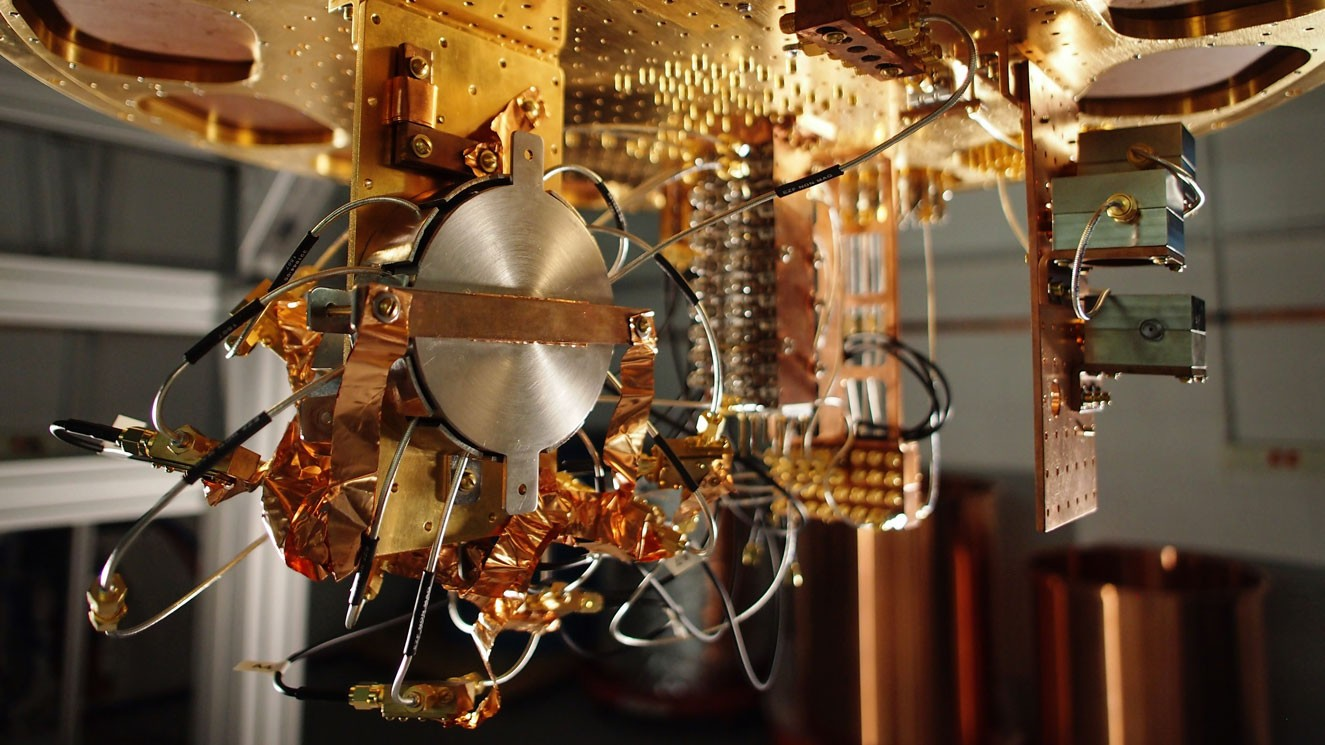
\includegraphics[width=\linewidth, height=1.5in, keepaspectratio]{../figure/googlequantum.jpg}
\caption{Superconducting quantum computer prototype at Google. Image
credit: Google / MIT Technology Review.}
\label{googlequantumfig}
\end{marginfigure}

There have been several proposals to build quantum computers:

\begin{itemize}
\item
  \href{https://en.wikipedia.org/wiki/Superconducting_quantum_computing}{Superconducting
  quantum computers} use superconducting electric circuits to do quantum
  computation. This is the direction where
  \href{https://arxiv.org/abs/1709.06678}{there has been most recent
  progress} towards ``beating'' classical computers.
\item
  \href{https://en.wikipedia.org/wiki/Trapped_ion_quantum_computer}{Trapped
  ion quantum computers} Use the states of an ion to simulate a qubit.
  People have made some
  \href{http://iontrap.umd.edu/wp-content/uploads/2016/02/1602.02840v1.pdf}{recent
  advances} on these computers too. While it's not at all clear that's
  the right measuring yard, the
  \href{http://arxiv.org/abs/1507.08852}{current best implementation} of
  Shor's algorithm (for factoring 15) is done using an ion-trap
  computer.
\item
  \href{https://en.wikipedia.org/wiki/Topological_quantum_computer}{Topological
  quantum computers} use a different technology. Topological qubits are
  more stable by design and hence error correction is less of an issue,
  but constructing them is extremely challenging.
\end{itemize}

These approaches are not mutually exclusive and it could be that
ultimately quantum computers are built by combining all of them
together. In the near future, it seems that we will not be able to
achieve full fledged large scale universal quantum computers, but rather
more restricted machines, sometimes called ``Noisy Intermediate-Scale
Quantum Computers'' or ``NISQ''. See
\href{https://arxiv.org/abs/1801.00862}{this article by John Preskil}
for some of the progress and applications of such more restricted
devices.

\section{Shor's Algorithm: Hearing the shape of prime
factors}\label{Shors-Algorithm-Hearing-t}

Bell's Inequality is a powerful demonstration that there is something
very strange going on with quantum mechanics. But could this
``strangeness'' be of any use to solve computational problems not
directly related to quantum systems? A priori, one could guess the
answer is \emph{no}. In 1994 Peter Shor showed that one would be wrong:

\hypertarget{shorthm}{}
\begin{theorem}[Shor's Algorithm] \label[theorem]{shorthm}

There is a polynomial-time quantum algorithm that on input an integer
\(M\) (represented in base two), outputs the prime factorization of
\(M\).

\end{theorem}

Another way to state \cref{shorthm} is that if we define
\(\ensuremath{\mathit{FACTORING}}:\{0,1\}^* \rightarrow \{0,1\}\) to be
the function that on input a pair of numbers \((M,X)\) outputs \(1\) if
and only if \(M\) has a factor \(P\) such that \(2 \leq P \leq X\), then
\(\ensuremath{\mathit{FACTORING}}\) is in \(\mathbf{BQP}\). This is an
exponential improvement over the best known classical algorithms, which
take roughly \(2^{\tilde{O}(n^{1/3})}\) time, where the \(\tilde{O}\)
notation hides factors that are polylogarithmic in \(n\). While we will
not prove \cref{shorthm} in this chapter, we will sketch some of the
ideas behind the proof.

\subsection{Period finding}\label{Period-finding}

At the heart of Shor's Theorem is an efficient quantum algorithm for
finding \emph{periods} of a given function. For example, a function
\(f:\R \rightarrow \R\) is \emph{periodic} if there is some \(h>0\) such
that \(f(x+h)=f(x)\) for every \(x\) (e.g., see \cref{periodicfig}).


\begin{marginfigure}
\centering
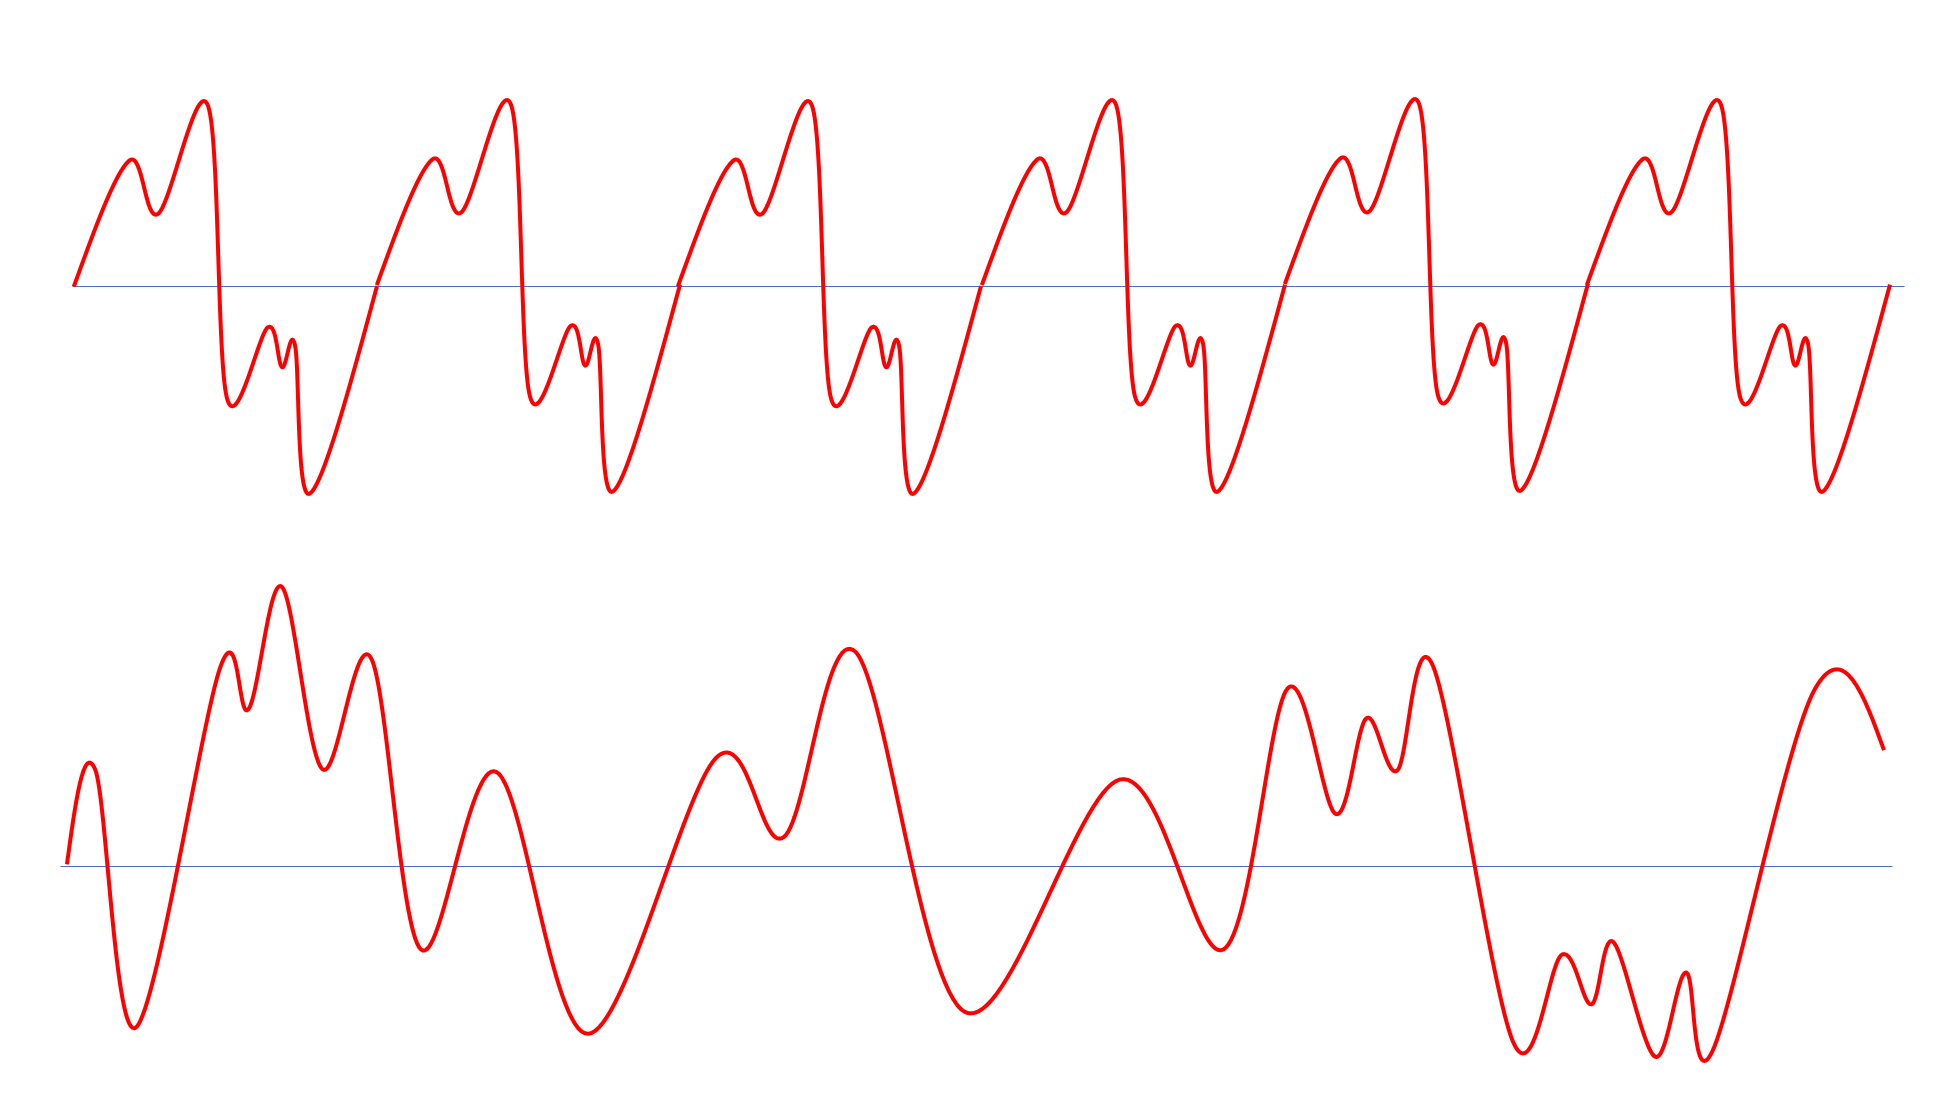
\includegraphics[width=\linewidth, height=1.5in, keepaspectratio]{../figure/periodic_vs_aperiodic.png}
\caption{Top: A periodic function. Bottom: An a-periodic function.}
\label{periodicfig}
\end{marginfigure}

\emph{Musical notes} yield one type of periodic function. When you pull
on a string on a musical instrument, it vibrates in a repeating pattern.
Hence, if we plot the speed of the string (and so also the speed of the
air around it) as a function of time, it will correspond to some
\emph{periodic} function. The length of the period is known as the
\emph{wave length} of the note. The \emph{frequency} is the number of
times the function repeats itself within a unit of time. For example,
the ``Middle C'' note has a frequency of \(261.63\) Hertz, which means
its period is \(1/(261.63)\) seconds.

If we play a \emph{chord} by playing several notes at once, we get a
more complex periodic function obtained by combining the functions of
the individual notes (see \cref{timefreqfig}). The human ear contains
many small hairs, each of which is sensitive to a narrow band of
frequencies. Hence when we hear the sound corresponding to a chord, the
hairs in our ears actually separate it out to the components
corresponding to each frequency.


\begin{marginfigure}
\centering
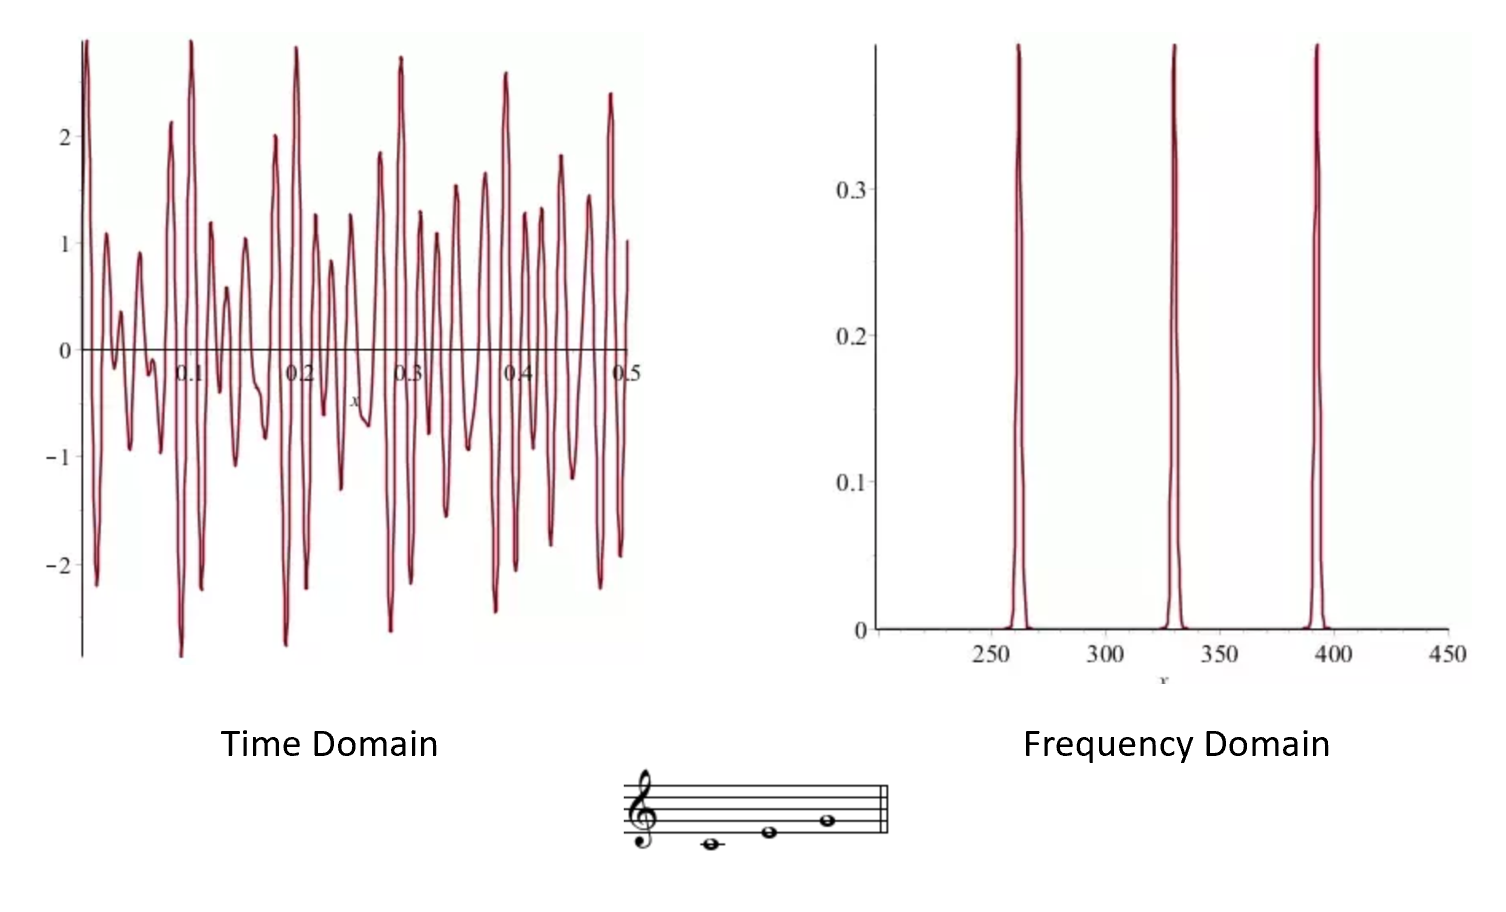
\includegraphics[width=\linewidth, height=1.5in, keepaspectratio]{../figure/timefreq.png}
\caption{Left: The air-pressure when playing a ``C Major'' chord as a
function of time. Right: The coefficients of the Fourier transform of
the same function, we can see that it is the sum of three frequencies
corresponding to the C, E and G notes (261.63, 329.63 and 392 Hertz
respectively). Credit: Bjarke Mønsted's
\href{https://www.quora.com/What-is-the-meaning-of-frequency-domain}{Quora
answer}.}
\label{timefreqfig}
\end{marginfigure}

It turns out that (essentially) \emph{every} periodic function
\(f:\R \rightarrow \R\) can be decomposed into a sum of simple
\emph{wave} functions (namely functions of the form
\(x \mapsto \sin(\theta x)\) or \(x \mapsto \cos(\theta x)\)). This is
known as the
\href{https://en.wikipedia.org/wiki/Fourier_transform}{Fourier
Transform} (see \cref{qfourierfig}). The Fourier transform makes it easy
to compute the period of a given function: it will simply be the least
common multiple of the periods of the constituent waves.


\begin{marginfigure}
\centering
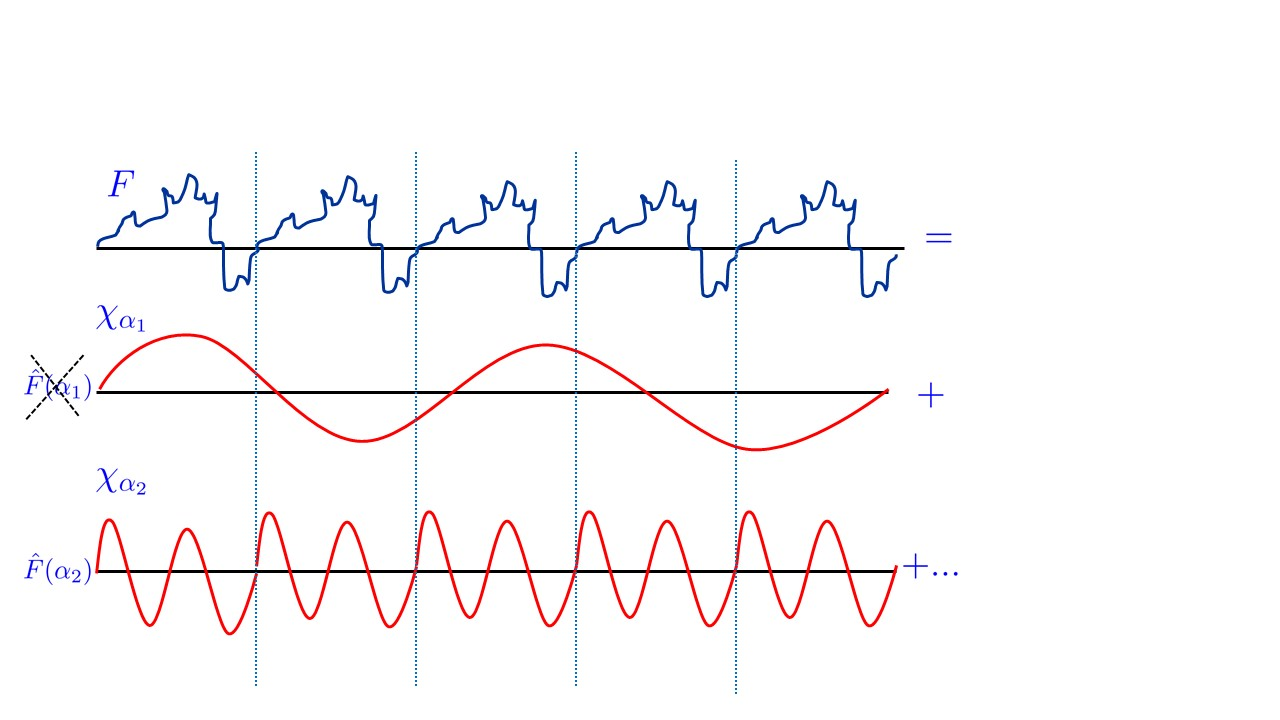
\includegraphics[width=\linewidth, height=1.5in, keepaspectratio]{../figure/quantum_fourier.jpg}
\caption{If \(f\) is a periodic function then when we represent it in
the Fourier transform, we expect the coefficients corresponding to
wavelengths that do not evenly divide the period to be very small, as
they would tend to ``cancel out''.}
\label{qfourierfig}
\end{marginfigure}

\subsection{Shor's Algorithm: A bird's eye
view}\label{Shors-Algorithm-A-birds-e}

On input an integer \(M\), Shor's algorithm outputs the prime
factorization of \(M\) in time that is polynomial in \(\log M\). The
main steps in the algorithm are the following:

\paragraph{Step 1: Reduce to period finding.} The first step in the
algorithm is to pick a random \(A\in \{0,1\ldots,M-1\}\) and define the
function \(F_A:\{0,1\}^m \rightarrow \{0,1\}^m\) as
\(F_A(x)= A^x (\mod M)\) where we identify the string
\(x \in \{0,1\}^m\) with an integer using the binary representation, and
similarly represent the integer \(A^x (\mod M)\) as a string. (We will
choose \(m\) to be some polynomial in \(\log M\) and so in particular
\(\{0,1\}^m\) is a large enough set to represent all the numbers in
\(\{0,1,\ldots, M-1 \}\)).

Some not-too-hard (though somewhat technical) calculations show that:
\textbf{(1)} The function \(F_A\) is \emph{periodic} (i.e., there is
some integer \(p_A\) such that \(F_A(x+p_A)=F_A(x)\) for ``almost''
every \(x\)) and more importantly \textbf{(2)} If we can recover the
period \(p_A\) of \(F_A\) for several randomly chosen \(A\)'s, then we
can recover the factorization of \(M\). (We'll ignore the ``almost''
qualifier in the discussion below; it causes some annoying, yet
ultimately manageable, technical issues in the full-fledged algorithm.)
Hence, factoring \(M\) reduces to finding out the period of the function
\(F_A\). \cref{dlogfromorder} asks you to work out this for the related
task of computing the \emph{discrete logarithm} (which underlies the
security of the Diffie-Hellman key exchange and elliptic curve
cryptography).

\paragraph{Step 2: Period finding via the Quantum Fourier Transform.}
Using a simple trick known as ``repeated squaring'', it is possible to
compute the map \(x \mapsto F_A(x)\) in time polynomial in \(m\), which
means we can also compute this map using a polynomial number of NAND
gates,and so in particular we can generate in polynomial quantum time a
quantum state \(\rho\) that is (up to normalization) equal to

\[
\sum_{x\in \{0,1\}^m} |x\rangle |F_A(x) \rangle \;\;.
\]

In particular, if we were to \emph{measure} the state \(\rho\), we would
get a random pair of the form \((x,y)\) where \(y= F_A(x)\). So far,
this is not at all impressive. After all, we did not need the power of
quantum computing to generate such pairs: we could simply generate a
random \(x\) and then compute \(F_A(x)\).

Another way to describe the state \(\rho\) is that the coefficient of
\(|x \rangle |y \rangle\) in \(\rho\) is proportional to \(f_{A,y}(x)\)
where \(f_{A,y} : \{0,1\}^m \rightarrow \R\) is the function such that
\[f_{A,y}(x) = \begin{cases} 1 & y = A^x (\mod M) \\ 0 & \text{otherwise} \end{cases} \;.\]

The magic of Shor's algorithm comes from a procedure known as the
\href{https://en.wikipedia.org/wiki/Quantum_Fourier_transform}{\emph{Quantum
Fourier Transform}}. It allows to change the state \(\rho\) into the
state \(\hat{\rho}\) where the coefficient of \(|x\rangle|y \rangle\) is
now proportional to the \emph{\(x\)-th Fourier coefficient} of
\(f_{A,y}\). In other words, if we measure the state \(\hat{\rho}\), we
will obtain a pair \((x,y)\) such that the probability of choosing \(x\)
is proportional to the square of the weight of the \emph{frequency}
\(x\) in the representation of the function \(f_{A,y}\). Since for every
\(y\), the function \(f_{A,y}\) has the period \(p_A\), it can be shown
that the frequency \(x\) will be (almost) a multiple of \(p_A\). If we
make several such samples \(y_0,\ldots,y_k\) and obtain the frequencies
\(x_1,\ldots,x_k\), then the true period \(p_A\) divides all of them,
and it can be shown that it is going to be in fact the \emph{greatest
common divisor} (g.c.d.) of all these frequencies: a value which can be
computed in polynomial time.

As mentioned above, we can recover the factorization of \(M\) from the
periods of \(F_{A_0},\ldots,F_{A_t}\) for some randomly chosen
\(A_0,\ldots,A_t\) in \(\{0,\ldots, M-1\}\) and \(t\) which is
polynomial in \(\log M\).

The resulting algorithm can be described in a high (and somewhat
inaccurate) level as follows:

\begin{quote} \label[quote]{Shors-Algorithm-sketchInp}

\textbf{Shor's Algorithm:} \emph{(sketch)}

\textbf{Input:} Number \(M\in \N\).

\textbf{Output:} Prime factorization of \(M\).

\textbf{Operations:}

\begin{enumerate}
\def\labelenumi{\arabic{enumi}.}
\item
  Repeat the following \(k=poly(\log M)\) number of times:

  \begin{enumerate}
  \def\labelenumii{\alph{enumii}.}
  \item
    Choose \(A \in \{0,\ldots,M-1\}\) at random, and let
    \(f_A:\Z_M \rightarrow \Z_M\) be the map \(x \mapsto A^x \mod M\).
  \item
    For \(t=poly(\log M)\), repeat \(t\) times the following step:
    \emph{Quantum Fourier Transform} to create a quantum state
    \(| \psi \rangle\) over \(poly(\log(m))\) qubits, such that if we
    measure \(| \psi \rangle\) we obtain a pair of strings \((j,y)\)
    with probability proportional to the square of the coefficient
    corresponding to the wave function \(x \mapsto \cos(x \pi j/M)\) or
    \(x \mapsto \sin(x \pi j/M)\) in the Fourier transform of the
    function \(f_{A,y}:\Z_m \rightarrow \{0,1\}\) defined as
    \(f_{A,y}(x)=1\) iff \(f_A(x)=y\).
  \item
    If \(j_1,\ldots,j_t\) are the coefficients we obtained in the
    previous step, then the least common multiple of
    \(M/j_1,\ldots,M/j_t\) is likely to be the \emph{period} of the
    function \(f_A\).
  \end{enumerate}
\item
  If we let \(A_0,\ldots,A_{k-1}\) and \(p_0,\ldots,p_{k-1}\) be the
  numbers we chose in the previous step and the corresponding periods of
  the functions \(f_{A_0},\ldots,f_{A_{k-1}}\) then we can use classical
  results in number theory to obtain from these a non-trivial prime
  factor \(Q\) of \(M\) (if such exists). We can now run the algorithm
  again with the (smaller) input \(M/Q\) to obtain all other factors.
\end{enumerate}

\end{quote}

Reducing factoring to order finding is cumbersome, but can be done in
polynomial time using a classical computer. The key quantum ingredient
in Shor's algorithm is the \emph{quantum fourier transform}.

\hypertarget{QFT}{}
\begin{remark}[Quantum Fourier Transform] \label[remark]{QFT}

Despite its name, the Quantum Fourier Transform does \emph{not} actually
give a way to compute the Fourier Transform of a function
\(f:\{0,1\}^m \rightarrow \R\). This would be impossible to do in time
polynomial in \(m\), as simply writing down the Fourier Transform would
require \(2^m\) coefficients. Rather the Quantum Fourier Transform gives
a \emph{quantum state} where the amplitude corresponding to an element
(think: frequency) \(h\) is equal to the corresponding Fourier
coefficient. This allows to sample from a distribution where \(h\) is
drawn with probability proportional to the square of its Fourier
coefficient. This is not the same as computing the Fourier transform,
but is good enough for recovering the period.

\end{remark}

\section{Quantum Fourier Transform (advanced,
optional)}\label{Quantum-Fourier-Transform}

The above description of Shor's algorithm skipped over the
implementation of the main quantum ingredient: the \emph{Quantum Fourier
Transform} algorithm. In this section we discuss the ideas behind this
algorithm. We will be rather brief and imprecise.
\cref{quantumbibnotessec} contain references to sources of more
information about this topic.

To understand the Quantum Fourier Transform, we need to better
understand the Fourier Transform itself. In particular, we will need to
understand how it applies not just to functions whose input is a real
number but to functions whose domain can be any arbitrary commutative
\emph{group}. Therefore we now take a short detour to (very basic)
\emph{group theory}, and define the notion of periodic functions over
groups.

\hypertarget{grouptheorem}{}
\begin{remark}[Group theory] \label[remark]{grouptheorem}

While we define the concepts we use, some background in group or number
theory will be very helpful for fully understanding this section. In
particular we will use the notion of \emph{finite commutative (a.k.a.
Abelian) groups}. These are defined as follows.

\begin{itemize}
\item
  A finite \emph{group} \(\mathbb{G}\) is a pair \((G,\star)\) where
  \(G\) is a finite set of elements and \(\star\) is a \emph{binary
  operation} mapping a pair \(g,h\) of elements in \(G\) to the element
  \(g \star h\) in \(G\). We often identify \(\mathbb{G}\) with the set
  \(G\) of its elements, and so use notation such as \(g\in \mathbb{G}\)
  to indicate that \(g\) is an element of \(\mathbb{G}\) and
  \(|\mathbb{G}|\) to denote the number of elements in \(\mathbb{G}\).
\item
  The operation \(\star\) satisfies the sort of properties that a
  product operation does, namely, it is \emph{associative} (i.e.,
  \((g \star h)\star f = g \star (h \star f)\)) and there is some
  element \(1\) such that \(g \star 1 = g\) for all \(g\), and for every
  \(g\in \mathbb{G}\) there exists an element \(g^{-1}\) such that
  \(g \star g^{-1} = 1\).
\item
  A group is called \emph{commutative} (also known as \emph{Abelian}) if
  \(g \star h = h \star g\) for all \(g,h \in \mathbb{G}\).
\end{itemize}

\end{remark}

The Fourier transform is a deep and vast topic, on which we will barely
touch upon here. Over the real numbers, the Fourier transform of a
function \(f\) is obtained by expressing \(f\) in the form
\(\sum \hat{f}(\alpha)\chi_\alpha\) where the \(\chi_\alpha\)'s are
``wave functions'' (e.g.~sines and cosines). However, it turns out that
the same notion exists for \emph{every} Abelian group \(\mathbb{G}\).
Specifically, for every such group \(\mathbb{G}\), if \(f\) is a
function mapping \(\mathbb{G}\) to \(\mathbb{C}\), then we can write
\(f\) as

\[f = \sum_{g \in \mathbb{G}} \hat{f}(g)\chi_g \;\;, \label{fourierexpansion}\]

where the \(\chi_g\)'s are functions mapping \(\mathbb{G}\) to
\(\mathbb{C}\) that are analogs of the ``wave functions'' for the group
\(\mathbb{G}\) and for every \(g\in \mathbb{G}\), \(\hat{f}(g)\) is a
complex number known as the \emph{Fourier coefficient of \(f\)
corresponding to \(g\)}. Specifically, the equation
\eqref{fourierexpansion} means that if we think of \(f\) as a
\(|\mathbb{G}|\) dimensional vector over the complex numbers, then we
can write this vector as a sum (with certain coefficients) of the
vectors \(\{ \chi_g \}_{g\in \mathbb{G}}\). The representation
\eqref{fourierexpansion} is known as the \emph{Fourier expansion} or
\emph{Fourier transform} of \(f\), the numbers
\(( \hat{f}(g) )_{g\in\mathbb{G}}\) are known as the \emph{Fourier
coefficients} of \(f\) and the functions \(( \chi_g )_{g\in\mathbb{G}}\)
are known as the \emph{Fourier characters}. The central property of the
Fourier characters is that they are \emph{homomorphisms} of the group
into the complex numbers, in the sense that for every
\(x,x' \in \mathbb{G}\), \(\chi_g(x \star x')=\chi_g(x)\chi_g(x')\),
where \(\star\) is the group operation. One corollary of this property
is that if \(\chi_g(h)=1\) then \(\chi_g\) is \emph{\(h\) periodic} in
the sense that \(\chi_g(x \star h)=\chi_g(x)\) for every \(x\). It turns
out that if \(f\) is periodic with minimal period \(h\), then the only
Fourier characters that have non zero coefficients in the expression
\eqref{fourierexpansion} are those that are \(h\) periodic as well. This
can be used to recover the period of \(f\) from its Fourier expansion.

\subsection{Quantum Fourier Transform over the Boolean Cube: Simon's
Algorithm}\label{Quantum-Fourier-Transform}

We now describe the simplest setting of the Quantum Fourier Transform:
the group \(\{0,1\}^n\) with the XOR operation, which we'll denote by
\((\{0,1\}^n,\oplus)\). (Since \(\ensuremath{\mathit{XOR}}\) is equal to
addition modulo two, this group is also often denoted as \((\Z_2)^n\).)
It can be shown that the Fourier transform over \((\{0,1\}^n,\oplus)\)
corresponds to expressing \(f:\{0,1\}^n \rightarrow \mathbb{C}\) as

\[
f = \sum_{y\in \{0,1\}} \hat{f}(y) \chi_y
\]

where \(\chi_y:\{0,1\}^n \rightarrow \mathbb{C}\) is defined as
\(\chi_y(x) = (-1)^{\sum_i y_i x_i}\) and
\(\hat{f}(y) = \tfrac{1}{\sqrt{2^n}}\sum_{x\in \{0,1\}^n} f(x)(-1)^{\sum_i y_i x_i}\).

The Quantum Fourier Transform over \((\{0,1\}^n,\oplus)\) is actually
quite simple:

\hypertarget{QFTcube}{}
\begin{theorem}[QFT Over the Boolean Cube] \label[theorem]{QFTcube}

Let \(\rho = \sum_{x\in \{0,1\}^n} f(x)|x\rangle\) be a quantum state
where \(f:\{0,1\}^n \rightarrow \mathbb{C}\) is some function satisfying
\(\sum_{x\in \{0,1\}^n} |f(x)|^2 = 1\). Then we can use \(n\) gates to
transform \(\rho\) to the state

\[\sum_{y\in \{0,1\}^n} \hat{f}(y) |y \rangle\]

where \(f = \sum_{y} \hat{f}(y)\chi_y\) and
\(\chi_y:\{0,1\}^n \rightarrow \mathbb{C}\) is the function
\(\chi_y(x) = -1^{\sum x_iy_i}\).

\end{theorem}

\begin{proofidea} \label[proofidea]{The-idea-behind-the-proof}

The idea behind the proof is that the \emph{Hadamard} operation
corresponds to the \emph{Fourier transform} over the group \(\{0,1\}^n\)
(with the XOR operations). To show this, we just need to do the
calculations.

\end{proofidea}

\begin{proof}[Proof of \cref{QFTcube}] \label[proof]{We-can-express-the-Hadama}

We can express the Hadamard operation \(\ensuremath{\mathit{HAD}}\) as
follows:

\[ \ensuremath{\mathit{HAD}}|a\rangle = \tfrac{1}{\sqrt{2}}(|0\rangle+(-1)^a|1\rangle) \;.\]

We are given the state \[\rho = \sum_{x\in\{0,1\}^n} f(x)|x\rangle \;.\]

Now suppose that we apply the \(\ensuremath{\mathit{HAD}}\) operation to
each of the \(n\) qubits. We can see that we get the state

\[2^{-n/2}\sum_{x\in\{0,1\}^n}f(x)\prod_{i=0}^{n-1}(|0\rangle+(-1)^{x_i}|1\rangle) \;.
\]

We can now use the distributive law and open up a term of the form

\[f(x)\bigl(|0\rangle + (-1)^{x_0}|1\rangle\bigr) \cdots  \bigl(|0\rangle + (-1)^{x_{n-1}}|1\rangle\bigr)\]

to the following sum over \(2^n\) terms: \[
f(x) \sum_{y \in \{0,1\}^n} (-1)^{\sum y_ix_i}|y \rangle \;.
\]

(If you find the above confusing, try to work out explicitly this
calculation for \(n=3\); namely show that
\(\bigl(|0\rangle + (-1)^{x_0}|1 \rangle\bigr) \bigl(|0\rangle + (-1)^{x_1}|1 \rangle \bigr) \bigl(|0\rangle + (-1)^{x_2}|1 \rangle \bigr)\)
is the same as the sum over \(2^3\) terms
\(|000\rangle + (-1)^{x_2}|001\rangle + \cdots +(-1)^{x_0+x_1+x_2}|111\rangle\).)

By changing the order of summations, we see that the final state is

\[
\sum_{y \in \{0,1\}^n} 2^{-n/2}\bigl(\sum_{x\in \{0,1\}^n} f(x) (-1)^{\sum x_i y_i} \bigr) | y \rangle
\]

which exactly corresponds to \(\hat{\rho}\).

\end{proof}

\subsection{From Fourier to Period finding: Simon's Algorithm (advanced,
optional)}\label{From-Fourier-to-Period-fi}

Using \cref{QFTcube} it is not hard to get an algorithm that can recover
a string \(h^* \in \{0,1\}^n\) given a circuit that computes a function
\(F:\{0,1\}^n \rightarrow \{0,1\}^*\) that is \emph{\(h^*\) periodic} in
the sense that \(F(x)=F(x')\) for distinct \(x,x'\) if and only if
\(x' = x \oplus h^*\). The key observation is that if we compute the
state \(\sum_{x\in \{0,1\}^n} |x \rangle |F(x) \rangle\), and perform
the Quantum Fourier transform on the first \(n\) qubits, then we would
get a state such that the only basis elements with nonzero coefficients
would be of the form \(|y \rangle\) where

\[
\sum y_i h^*_i = 0 (\mod 2) \label{eq:periodbooleanqft}
\]

So, by measuring the state, we can obtain a sample of a random \(y\)
satisfying \eqref{eq:periodbooleanqft}. But since
\eqref{eq:periodbooleanqft} is a \emph{linear} equation modulo \(2\)
about the unknown \(n\) variables \(h^*_0,\ldots,h^*_{n-1}\), if we
repeat this procedure to get \(n\) such equations, we will have at least
as many equations as variables and (it can be shown that) this will
suffice to recover \(h^*\).

This result is known as
\href{https://en.wikipedia.org/wiki/Simon\%27s_problem}{Simon's
Algorithm}, and it preceded and inspired Shor's algorithm.

\subsection{From Simon to Shor (advanced,
optional)}\label{From-Simon-to-Shor-advanc}

\cref{QFTcube} seemed to really use the special bit-wise structure of
the group \(\{0,1\}^n\), and so one could wonder if it can be extended
to other groups. However, it turns out that we can in fact achieve such
a generalization.

The key step in Shor's algorithm is to implement the Fourier transform
for the group \(\Z_L\) which is the set of numbers \(\{0,\ldots,L-1\}\)
with the operation being addition modulo \(L\). In this case it turns
out that the Fourier characters are the functions
\(\chi_y(x) = \omega^{yx}\) where \(\omega = e^{2\pi i/L}\) (\(i\) here
denotes the complex number \(\sqrt{-1}\)). The \(y\)-th Fourier
coefficient of a function \(f:\Z_L \rightarrow \mathbb{C}\) is

\[\hat{f}(y) = \tfrac{1}{\sqrt{L}}\sum_{x\in \Z_L} f(x)\omega^{xy} \;. \label{fouriercoeffmodular}\]

The key to implementing the Quantum Fourier Transform for such groups is
to use the same recursive equations that enable the classical
\href{https://en.wikipedia.org/wiki/Fast_Fourier_transform}{Fast Fourier
Transform (FFT)} algorithm. Specifically, consider the case that
\(L=2^\ell\). We can separate the sum over \(x\) in
\eqref{fouriercoeffmodular} to the terms corresponding to even \(x\)'s
(of the form \(x=2z\)) and odd \(x\)'s (of the form \(x=2z+1\)) to
obtain

\[\hat{f}(y) = \tfrac{1}{\sqrt{L}}\sum_{z \in Z_{L/2}} f(2z)(\omega^2)^{yz} + \tfrac{\omega^y}{\sqrt{L}}\sum_{z\in \Z_{L/2}}f(2z+1)(\omega^2)^{yz} \label{eqfftrecurse}
\]

which reduces computing the Fourier transform of \(f\) over the group
\(\Z_{2^\ell}\) to computing the Fourier transform of the functions
\(f_{even}\) and \(f_{odd}\) (corresponding to the applying \(f\) to
only the even and odd \(x\)'s respectively) which have \(2^{\ell-1}\)
inputs that we can identify with the group \(\Z_{2^{\ell-1}}=\Z_{L/2}\).

Specifically, the Fourier characters of the group \(\Z_{L/2}\) are the
functions \(\chi_y(x) = e^{2\pi i/(L/2) yx} = (\omega^2)^{yx}\) for
every \(x,y \in \Z_{L/2}\). Moreover, since \(\omega^L = 1\),
\((\omega^2)^y = (\omega^2)^{y \mod L/2}\) for every \(y\in \N\). Thus
\eqref{eqfftrecurse} translates into
\[\hat{f}(y) = \hat{f}_{even}(y \mod L/2) + \omega^y \hat{f}_{odd}(y \mod L/2) \;.
\]

This observation is usually used to obtain a fast (e.g.~\(O(L \log L)\))
time to compute the Fourier transform in a classical setting, but it can
be used to obtain a quantum circuit of \(poly(\log L)\) gates to
transform a state of the form \(\sum_{x\in \Z_L} f(x)|x\rangle\) to a
state of the form \(\sum_{y\in \Z_L} \hat{f}(y)|y \rangle\).

The case that \(L\) is not an exact power of two causes some
complications in both the classical case of the Fast Fourier Transform
and the quantum setting of Shor's algorithm. However, it is possible to
handle these. The idea is that we can embed \(Z_L\) in the group
\(\Z_{A\cdot L}\) for any integer \(A\), and we can find an integer
\(A\) such that \(A\cdot L\) will be close enough to a power of \(2\)
(i.e., a number of the form \(2^m\) for some \(m\)), so that if we do
the Fourier transform over the group \(\Z_{2^m}\) then we will not
introduce too many errors.


\begin{figure}
\centering
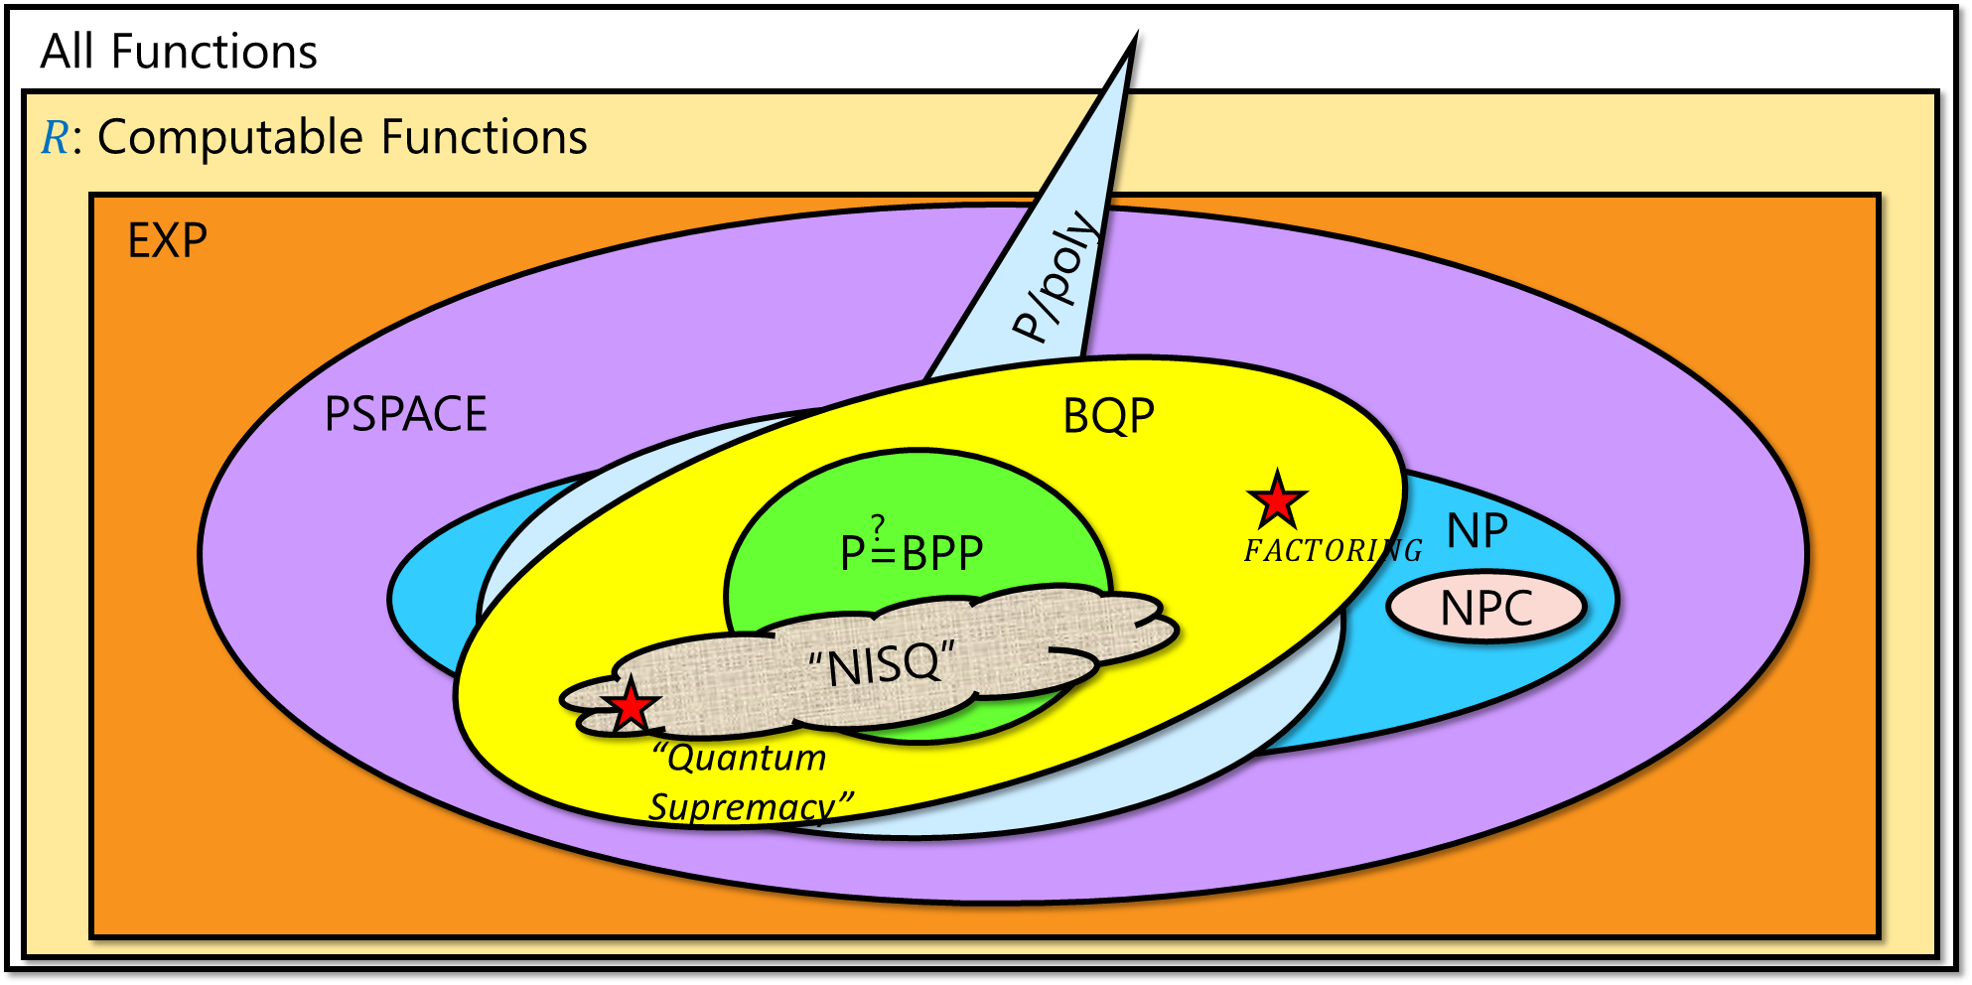
\includegraphics[width=\textwidth, height=0.25\paperheight, keepaspectratio]{../figure/quantumscenarios.png}
\caption{Conjectured status of \(\mathbf{BQP}\) with respect to other
complexity classes. We know that
\(\mathbf{P} \subseteq \mathbf{BPP} \subseteq \mathbf{BQP}\) and
\(\mathbf{BQP} \subseteq \mathbf{PSPACE} \subseteq \mathbf{EXP}\). It is
not known if any of these inclusions are strict though it is believed
that they are. The relation between \(\mathbf{BQP}\) and \(\mathbf{NP}\)
is unknown but they are believed to be incomparable, and that
\(\mathbf{NP}\)-complete problems \emph{can not} be solved in polynomial
time by quantum computers. However, it is possible that \(\mathbf{BQP}\)
contains \(\mathbf{NP}\) and even \(\mathbf{PSPACE}\), and it is also
possible that quantum computers offer no super-polynomial speedups and
that \(\mathbf{P}=\mathbf{BQP}\). The class ``\(\mathbf{NISQ}\)'' above
is not a well defined complexity class, but rather captures the current
status of quantum devices, which seem to be able to solve a set of
computational tasks that is incomparable with the set of tasks solvable
by classical computers. The diagram is also inaccurate in the sense that
at the moment the ``quantum supremacy'' tasks on which such devices seem
to offer exponential speedups do \emph{not} correspond to Boolean
functions/ decision problems.}
\label{quantumoptionsfig}
\end{figure}

\begin{recap} \label[recap]{The-state-of-an-n-qubit-q}

\begin{itemize}
\tightlist
\item
  The state of an \(n\)-qubit quantum system can be modeled as a \(2^n\)
  dimensional vector
\item
  An operation on the state corresponds to applying a unitary matrix to
  this vector.
\item
  Quantum circuits are obtained by composing basic operations such as
  \(\ensuremath{\mathit{HAD}}\) and \(U_{NAND}\).
\item
  We can use quantum circuits to define the classes
  \(\mathbf{BQP_{/poly}}\) and \(\mathbf{BQP}\) which are the quantum
  analogs of \(\mathbf{P_{/poly}}\) and \(\mathbf{BPP}\) respectively.
\item
  There are some problems for which the best known quantum algorithm is
  \emph{exponentially faster} than the best known, but quantum computing
  is not a panacea. In particular, as far as we know, quantum computers
  could still require exponential time to solve \(\mathbf{NP}\)-complete
  problems such as \(\ensuremath{\mathit{SAT}}\).
\end{itemize}

\end{recap}

\section{Exercises}\label{Exercises}

\hypertarget{BQPcontainements}{}
\begin{exercise}[Quantum and classical complexity class relations] \label[exercise]{BQPcontainements}

Prove the following relations between quantum complexity classes and
classical ones:

\begin{enumerate}
\def\labelenumi{\arabic{enumi}.}
\item
  \(\mathbf{P_{/poly}} \subseteq \mathbf{BQP_{/poly}}\). See footnote
  for hint.\footnote{You can use \(U_{NAND}\) to simulate NAND gates.}
\item
  \(\mathbf{P} \subseteq \mathbf{BQP}\). See footnote for
  hint.\footnote{Use the alternative characterization of \(\mathbf{P}\)
    as in \cref{Palternativeex}.}
\item
  \(\mathbf{BPP} \subseteq \mathbf{BQP}\). See footnote for
  hint.\footnote{You can use the \(\ensuremath{\mathit{HAD}}\) gate to
    simulate a coin toss.}
\item
  \(\mathbf{BQP} \subseteq \mathbf{EXP}\). See footnote for
  hint.\footnote{In exponential time simulating quantum computation
    boils down to matrix multiplication.}
\item
  If \(\ensuremath{\mathit{SAT}} \in \mathbf{BQP}\) then
  \(\mathbf{NP} \subseteq \mathbf{BQP}\). See footnote for
  hint.\footnote{If a reduction can be implemented in \(\mathbf{P}\) it
    can be implemented in \(\mathbf{BQP}\) as well.}
\end{enumerate}

\end{exercise}

\hypertarget{dlogfromorder}{}
\begin{exercise}[Discrete logarithm from order finding] \label[exercise]{dlogfromorder}

Show a probabilistic polynomial time classical algorithm that given an
Abelian finite group \(\mathbb{G}\) (in the form of an algorithm that
computes the group operation), a \emph{generator} \(g\) for the group,
and an element \(h \in \mathbb{G}\), as well as access to a black box
that on input \(f\in \mathbb{G}\) outputs the \emph{order} of \(f\) (the
smallest \(a\) such that \(f^a =1\)), computes the \emph{discrete
logarithm} of \(h\) with respect to \(g\). That is the algorithm should
output a number \(x\) such that \(g^x = h\). See footnote for
hint.\footnote{We are given \(h=g^x\) and need to recover \(x\). To do
  so we can compute the order of various elements of the form
  \(h^ag^b\). The order of such an element is a number \(c\) satisfying
  \(c(xa+b) = 0 \pmod{|\mathbb{G}|}\). With a few random examples we
  will get a non trivial equation on \(x\) (where \(c\) is not zero
  modulo \(|\mathbb{G}|\)) and then we can use our knowledge of
  \(a,b,c\) to recover \(x\).}

\end{exercise}

\section{Bibliographical notes}\label{quantumbibnotessec}

An excellent gentle introduction to quantum computation is given in
Mermin's book \cite{mermin2007quantum}. In particular the first 100
pages (Chapter 1 to 4) of \cite{mermin2007quantum} cover all the
material of this chapter in a much more comprehensive way. This material
is also covered in the first 5 chapters of
\href{https://arxiv.org/abs/1907.09415}{De-Wolf's online lecture notes}.
For a more condensed exposition, the chapter on quantum computation in
my \href{http://theory.cs.princeton.edu/complexity/}{book with Arora}
(see
\href{http://theory.cs.princeton.edu/complexity/ab_quantumchap.pdf}{draft
here}) is one relatively short source that contains full descriptions of
Grover's, Simon's and Shor's algorithms. This
\href{http://www.scottaaronson.com/blog/?p=208}{blog post of Aaronson}
contains a high level explanation of Shor's algorithm which ends with
links to several more detailed expositions. Chapters 9 and 10 in
Aaronson's book \cite{Aaronson13democritus} give an informal but highly
informative introduction to the topics of this chapter and much more.
Chapter 10 in \href{https://www.math.ias.edu/avi/book}{Avi Wigderson's
book} also provides a high level overview of quantum computing. Other
recommended resources include Andrew Childs'
\href{http://www.cs.umd.edu/~amchilds/qa/qa.pdf}{lecture notes on
quantum algorithms}, as well as the lecture notes of
\href{https://inst.eecs.berkeley.edu/~cs191/}{Umesh Vazirani},
\href{http://www.theory.caltech.edu/people/preskill/ph229/}{John
Preskill}, and
\href{https://cs.uwaterloo.ca/~watrous/LectureNotes.html}{John Watrous}.

There are many excellent videos available online covering some of these
materials. The videos of
\href{https://www.youtube.com/playlist?list=PLDAjb_zu5aoFazE31_8yT0OfzsTcmvAVg}{Umesh
Vazirani'z EdX course} are an accessible and recommended introduction to
quantum computing. Regarding quantum mechanics in general, this
\href{https://www.youtube.com/watch?v=DfPeprQ7oGc}{video} illustrates
the double slit experiment, this
\href{https://www.youtube.com/watch?v=xM3GOXaci7w}{Scientific American
video} is a nice exposition of Bell's Theorem. This
\href{https://youtu.be/GdqC2bVLesQ?t=2m51s}{talk and panel} moderated by
Brian Greene discusses some of the philosophical and technical issues
around quantum mechanics and its so called ``measurement problem''. The
\href{http://www.feynmanlectures.caltech.edu/I_50.html}{Feynmann lecture
on the Fourier Transform} and
\href{http://www.feynmanlectures.caltech.edu/III_toc.html}{quantum
mechanics in general} are very much worth reading. The Fourier transform
is covered in these videos of
\href{https://youtu.be/EYRmB1aNh9I?t=19s}{Dr.~Chris Geoscience},
\href{https://www.youtube.com/watch?v=Y9pYHDSxc7g}{Clare Zhang} and
\href{https://www.youtube.com/watch?v=i_0DXxNeaQ0}{Vi Hart}. See also
\href{https://www.youtube.com/watch?v=wUwZZaI5u0c}{Kelsey
Houston-Edwards's video on Shor's Algorithm}.

The form of Bell's game we discuss in \cref{bellineqsec} was given by
\href{https://goo.gl/wvJGZU}{Clauser, Horne, Shimony, and Holt}.

The \href{https://en.wikipedia.org/wiki/Fast_Fourier_transform}{Fast
Fourier Transform}, used as a component in Shor's algorithm, is one of
the most widely used algorithms invented. The stories of its discovery
by Gauss in trying to calculate asteroid orbits and rediscovery by Tukey
during the cold war are fascinating as well.

The image in \cref{doubleslitfig} is taken from Wikipedia.

Thanks to Scott Aaronson for many helpful comments about this chapter.
